\chapter{进程与线程}
\thispagestyle{empty}

	我们现在开始更加细节化地讨论操作系统是如何设计和构建的。对于任何操作系统而言,最核心的概念是:进程,一个正在运行的程序抽象。所有的其他事情都是基于这个概念的,操作系统的设计者(以及学生)应该尽快地了解什么是进程的概念。进程是操作系统提供的最古老和最重要的抽象。
	他们支持并发的多个操作即使在只有一个CPU的情况下。他们将一个CPU转化为多个虚拟的CPU。没有进程抽象,现代计算将不复存在。在本章中我们将深入探讨关于进程和线程的细节。
	
	\section{进程}
	
	所有的现代计算机都在同时做一个事情。人们之前使用计算机可能还没有充分意识到这个事实,所以再使用一些例子将这个情况讲清楚一些。首先考虑一个Web服务器,来自各地的请求都在请求网页。
	当一个请求来的时候,服务器检查是否将所需要的页面是否在cache中。如果是,则将其发回;如果不是,则启动一个磁盘请求去取它。但是,从CPU的角度来看,磁盘请求需要漫长的时间。当等待一个磁盘请求结束的时候,更多的请求可能会产生。如果有多个磁盘存在,一些或所有较新的磁盘可能在第一个请求得到满足之前就被发送到其他磁盘。很清楚,需要一些方法来建模和控制并发性。进程可以起到作用(特别是线程)。
	现在考虑一下用户的PC,当系统启动了以后,许多进程就无声无息地被启动了,尽管用户自己可能都不知道。例如,一个进程可能会被启动用来接收邮件。另外一个进程可能正在运行一个反病毒的程序,并且周期性地检查是否有新的病毒出现。除此之外,可能还有一些显式的进程,打印文件或者向USB驱动器中备份用户的照片,与此同时,用户可能还在网上进行冲浪。所有的这些活动都需要被管理,因此一个支持多线程的多道程序就来的非常及时了。在任何的多道程序系统中,CPU非常快速地从一个进程切换到另外一个进程,运行每一个进程数十或数百个微秒。但是,严格地说,在任何一个时候CPU都只能运行一个程序。在1秒钟之内,它可能对好几个进程产生作用,给人一种并行的错觉。有时候人们称之为伪并行策略,和真正的硬件并行的多核操作系统相比(有两个或者更多的CPU共享同样的内存)。跟踪并行的,多核的活动对于人来说是非常困难的。所以,操作系统的设计者们这些年开始提出了一种概念模型(顺序线程),使得并发性更容易被处理。它使用的这个模型,以及一些结果组成了本章的主要内容。
	
	\subsection{进程模型}
	
	在这个模型中,所有可以被运行的软件,有时候包括操作系统本身,都被组织成若干个顺序进程(Sequential process),简称进程。一个进程是一个正在执行的程序的实例,包括程序计数器现有的值,寄存器和变量。概念性地,每一个CPU都有一个自己的虚拟CPU。事实上,当然,真正的CPU在进程与进程之间来回地切换,但是为了理解好系统,想象一下一组进程在并行地执行比跟踪CPU是如何从一个程序向另外一个程序切换的要容易地多。这种快速的来回切换称为多道程序设计,如我们在第1章中提到的那样。
	在图 \ref{fig:processconcept} (a)中,我们看到一台计算机在内存中同时运行四个程序。在图 \ref{fig:processconcept} (b)中,我们看到四个进程,每一个都有自己的控制流程(它自己的逻辑程序计数器),而且每一个都是互相之间独立运行的。当然,只有一个物理的程序计数器,所以当每一个进程运行的时候,它们的逻辑程序计数器就会被加载到真正的程序计数器中。
	
	\begin{figure}[ht]\small
		\centering
		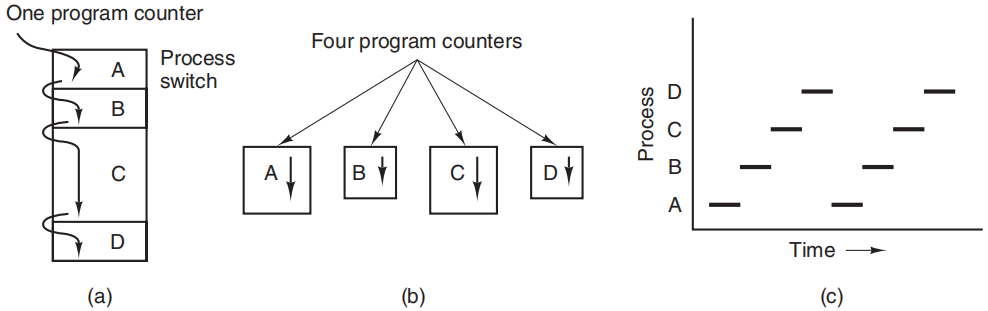
\includegraphics[width=0.85\textwidth]{FIG/2-1.png}
		\caption{a) 四个程序的多道程序 b) 四个独立的,顺序的概念模型 c) 只有一个程序在某一个时刻是活动的} \label{fig:processconcept}
	\end{figure}
	
	当程序结束的时候(时间到了),物理程序计数器保存在内存中的进程存储逻辑程序计数器中。从图 \ref{fig:processconcept} (c) 中我们可以看到,从一个足够长的时间间隔看,所有的进程都有进展,但是从一个给定的时间点来看,只有一个进程是实际运行的。在本章中,我们假设只有一个CPU。当然,逐渐这个假设就不为真了,因为新的芯片总是有多核的,有两个,四个,甚至更多的核。我们将在第8章中介绍多核芯片和多处理器。所以当我们说一个CPU一个时刻只能运行一个进程的时候,是指一个核心(一个CPU)在一个时刻只能运行一个进程。当CPU在进程之间来回切换的时候,一个进程执行其计算的速率将不一致,如果再次运行相同的进程,甚至可能无法再现以上的情形。所以,在对进程进行编程的时候,决不能对时序做任何想当然地假设。考虑一下,例如,一种播放音乐以伴随另一台设备运行的高质量视频的音频处理过程。
	因为音频一般会比视频稍微出现地晚一些,它向视频服务器发出信号开始播放,然后在回放音频之前运行一个空闲循环10000次。如果循环是一个可靠的计时器的话,一切都会变的OK,但是如果CPU决定在空闲循环的过程中切换到其他的线程,音频线程可能在相应的视频画面开始播放的时候还没有跟着播放出来,就会出现视频和音频不同步的恼人现象。当一个进程具有类似的关键性的实时需求,特定的事件必须在特定数值的毫秒内发生,则必须采取特定的措施来保障它确实能够按时发生。然而,通常情况下,大部分的进程是不受底层对CPU多道编程和不同的进程之间相对速度的影响的。进程与程序之间的区别是微不足道的,但是又是绝对关键的,一个模拟可能可以帮到你。考虑一下一个具有烹饪头脑的计算机科学家正在为他的年幼的女儿烤制生日蛋糕。他有一个生日蛋糕的菜单和具备所有输入食材的厨房:面粉,鸡蛋,糖,香草精等等。
	在这个模拟中,制作蛋糕的菜单就是程序(即用适当的形式描述的算法),计算机科学家是CPU,原材料是输入的数据。进程就是包括让烘焙机读取菜单,取原材料和烘焙蛋糕的过程。
	现在想象一下,这个时候计算机科学家的儿子捂着头哭着跑进来说他被蜜蜂给叮咬了。计算机科学家记录下当前菜单的状态(被保存的当前进程的状态),取出一本医疗救护手册,开始按照步骤处理蜜蜂蜇伤。这里我们看到,处理器从一个进程切(制作蛋糕)换到另外更高优先级的进程(进行医疗救治),每一个进程都有一个程序(菜单和急救手册)。当处理完蜜蜂蜇伤以后,计算机科学家又回来继续烘焙蛋糕,从他开始离开的时间点接着继续。关键的想法是一个进程是一种类型的活动。它有一个程序,一个输入,一个输出和一个状态。单个处理器可以被多个进程所共享,它使用某种调度算法来决定何时停止一个进程的工作并给另外一个进程提供服务。
	相反的是,程序就是存储在磁盘上的一段东西,它不做任何的事情。值得注意的是,如果一个程序被运行了两次,则它被视为是两个进程。例如,我们经常会同时启动两个文字处理软件,并在两个打印机同时可用的情况下同时打印两个文件。事实情况是,两个进程正好同时运行一个程序,这其实并不重要,因为他们是不同的进程。操作系统可以在他们之间共享代码,所以只需要在内存中存放一份代码,但是这只是一个技术细节,并不改变有两个进程运行的概念情况。
	
	\subsection{进程创建}
	
	操作系统需要一些方法来创建进程。在非常简单的系统中,或仅用于运行单个应用程序的系统(例如,微波炉中的控制器),当系统启动时,可能会出现所有需要的进程。在通用系统中,需要一些方法来创建和结束进程。我们将看一下一些可能的方法。四个原则性的事件将会导致进程被创建:
		1.) 系统初始化;
		2.) 一个正在运行的进程执行创建进程的系统调用;
		3.)	用户要求创建一个新的进程;
		4.) 批处理作业的初始化。
	当一个操作系统启动的时候,通常会创建若干个进程。其中有前台进程,这些进程和用户交互并为他们工作。剩下的一些运行在后台,不和特定的用户交互,但是有一些特定的功能。例如,一个后台进程可能会被设计用来接收新来的邮件,一天中的大部分时间在休眠,但是会在邮件到来的时候突然苏醒。另外一个后台进程可会被设计用来接收宿主机器的接收到的网页请求,在请求到来的时候苏醒并处理请求。用来处理类似邮件,网页,新闻,打印等任务的后台进程被称为守护进程(deamons)。大型的系统通常会有很多的守护进程。在UNIX\footnote{在本章中,应将UNIX理解为所有基于POSIX的操作系统,包括Linux,FreeBSD,OS X和Solaris等,甚至还包括Android和iOS等。}中,\texttt{ps}程序可以备用来列出正在运行的进程。在Windows中,可以使用任务管理器。
	
	除了在启动的时刻被创建的进程,进程还可以在后来被创建。通常一个运行的进程会调用系统调用来创建一个或者更多的进程来帮助它完成工作。创建新的进程会非常有用当所要完成的工作可以容易地被划分成几个相关的但是不互相作用的进程的时候。例如,一组大量的数据正在网络获取用来进行顺序处理,可以很方便地创建一个获取数据的进程,并把获取的数据放到一个共享缓冲区里,然后再创建一个进程来移动这些数据项并处理它们。在多处理器机中,可以允许每一个进程运行在不同的CPU上可以使工作处理地更快。
	
	在交互式系统中,用户可以通过键入一条命令或者点击(双击)一个图标来启动一个程序。这两个进程中的任何一个都会创建一个新的进程并在其中运行选择的程序。在基于命令行的UNIX系统中运行X,新的进程会从该进程接管它的窗口。在Windows中,当一个进程启动的时候它不会有一个窗口,但是它在运行的时候可以创建一个或多个窗口,而事实上它们大多也会这么做。在两个系统中,用户都可能同时打开多个窗口,并且运行一些进程。使用鼠标,用户可以选择一个窗口并进行进程交互,例如,在需要的时候提供输入。
	
	最后一种创建进程的情况是在大型机的批处理系统上。用户在这个系统中提交批处理作业。想象一下连锁店在一天结束的时候处理财务清单。这里用户可以提交批处理作业到系统(有可能是远程提交)。当操作系统觉得它有资源来运行其他的任务时,它创建一个新的进程并且从输入队列中运行下一个工作。
	
	技术上讲,在所有的这些情况下,一个新的进程通过现有的进程执行创建进程的系统调用来创建的。那个进程可以是正在运行的用户进程,一个从键盘或者鼠标触发的系统进程,或者是一个批管理进程。那个创建进程的进程所做的事情就是执行系统调用。系统调用告诉操作系统去创建一个新的进程并且直接或者间接地指定哪一个程序在其中运行。
	
	在UNIX中,只有一个系统调用可以创建一个新的进程:fork。这个调用创建一个调用进程的精确副本。在fork系统调用之后,父进程和子进程,拥有相同的内存镜像,相同的环境字符串,相同的打开文件。这就是全部的情形。通常情况下,子进程会执行execve系统调用或者一个类似的系统调用来改变其内存镜像和运行一个新的程序。例如,当用户键入一个命令:sort,给shell程序,shell产生一个子进程,子进程执行sort。此两步过程的原因是允许子进程在fork之后但在exece之前操作其文件描述符,以完成标准输入、标准输出和标准错误的重定向。
	
	在Windows中,对比之下,一个单个的Win32系统调用,CreateProcess,同时处理进程创建和将新的程序加载到进程中来。这个调用有10个参数,包括被执行的程序,喂给命令行程序的参数,不同的安全属性,控制继承是否被打开文件的位,优先信息,要为进程创建的窗口的规范(如果有),以及一个指向结构的指针,在该结构中,有关新创建的进程的信息将返回给调用者。除了\texttt{CreateProcess},Win32有差不多有100多个函数用于管理和同步进程以及其他的相关主题。
	
	在UNIX和Windows中,当一个进程被创建后,父进程和子进程有它们自己不同的地址空间。不管是哪一个地址空间改变了其地址空间的一个字节,这个变化对其他进程都是不可见的。在UNIX中,子进程的初始地址空间是父进程的一份复制,但是确实是有两个不同的地址空间,没有可写的内存是被共享的。一些UNIX实现方案在这两者之间共享程序文本,因为这两个都不能够被修改。相反地,子进程可以共享父进程的内存,但是在那种情况下内存是Copy-On-Write(写时复制)的,意味着无论是哪一个进程先修改那一部分内存,那一块的内存首先被显式地复制,并且保证修改出现在一个私有的内存区域上,这样,有没有可写的内存是共享的了。它是,然而,新创建的进程可以共享它的创建者的一些其他的资源,像打开文件。在Windows中,父进程和子进程的地址空间从一开始就是不一样的。
	
	\subsection{进程终止}
	
	在一个进程被创建后,它就开始运行并且开始工作了。但是,永恒是不存在的,即使进程也是这样。迟早一个新的进程会终止,通常是由以下情况造成的:
	1. 正常退出(自愿的)
	2. 错误退出(自愿的)
	3. 致命错误退出(非自愿的)
	4. 被其他进程杀死(非自愿的)
	多数进程是由于完成了它们的工作被终止。当一个编译器已经编译完给它的程序的时候,编译器就执行一个系统调用来告诉操作系统它完成了程序的编译。这个系统调用在UNIX中是exit,在Windows中是ExitProcess。面向屏幕的程序通常也支持志愿式退出。文件处理软件,因特网浏览器,还有一些其他相似的程序,总是有一个按钮或者菜单项,当用户点击的时候,告诉进程删除任何的它已经打开的暂时文件,并最终终止。终止的第二个原因是进程发现了一个致命的错误。例如,当一个用户键入命令:cc foo.c,来编译程序foo.c,但是这个程序又不存在,编译器简单地发现这个事实并退出了。面向画面的交互程序当给出错误参数的时候通常不会退出,相反它们会弹出一个对话框,让用户去重新试一下。停止一个进程的第三个原因是进程导致的错误,通常是由程序的错误造成的。例子包括执行了一个非法的指令,引用了不存在的内存或者进行了除零运算。在一些系统中(例如UNIX),一个进程可以告诉操作系统它想自己处理一些特定的错误,在这种情况下,当其中的一个错误出现的时候进程是被信号激活而不是终止。
	进程可能中止的第四个原因是进程执行一个系统调用来告诉操作系统杀死其他的进程。在UNIX中,这个系统调用是Kill,而Win32中相应的函数是TerminateProcess。在这两种情况下,执行杀死进程操作的进程都要获得一定的授权才可以进行操作。在一些系统中,当一个进程结束的时候,不管是非自愿地还是自愿地,所有该进程创建的其他进程也将被杀死。虽然说,UNIX和Windows都不是这样工作的。
	
	\subsection{进程层次}
	
	在一些系统中,当一个进程创建了其他的进程,父进程和子进程在很多方面还是相关联的,子进程本身也可以创建一些更多的进程,形成一个进程层次。注意到,不像动物和植物采用有性繁殖,一个进程只有一个父进程(但是可以有0个,1个,2个甚至更多个子进程)。所以,进程更像是一个多头蛇,或者说像一个母牛。在UNIX语言中,一个进程及其所有子进程和其他后代进程组成了一个进程组。当用户从键盘上发出一个信号的时候,信号被传送到当前与键盘关联的进程组的所有成员(通常是在当前窗口中创建的所有活动进程)。每一个进程都可以捕捉这个信号,或是忽略这个信号,或是采取相应的行动,即被该信号杀死。作为进程层次结构扮演着重要的角色的另一个例子,让我们看看在计算机启动之后,UNIX是如何初始化它自己的。一个称为\texttt{init}的特殊进程,出现在根镜像文件中。当它开始运行的时候,他读取一个文件告诉有多少个终端,然后为每一个终端分叉出一个新的进程。这些进程等待一些用户登录。如果一个登录成功了的话,登录进程执行一个shell来接收命令。这些命令可能会开启更多的进程。因此,所有系统的进程都被组织成了一个单个的进程树,而\texttt{init}进程是树根。相比而言,Windows就没有进程层次的概念。所有的进程都是平等的。唯一的关于进程层次的暗示是,当一个进程被创建的时候,进程被给予一个特殊的令牌(称为句柄),该令牌可以用来控制子进程。然而,它可以将句柄传递给其他进程,这样进程的层次结构就不存在了。在UNIX中,进程不能剥夺其子进程的"继承权"。
	
	\subsection{进程状态}
	
	尽管每一个进程都是一个独立的实体,有它自己的程序计数器和内部状态,进程通常还需要和其他进程进行交互。一个进程可能会产生一些其他进程用作输入的输出。在shell命令中,\texttt{cat chapter1 chapter2 chapter3 | grep tree},第一个进程运行cat,连接并输出三个文件。第二个进程,运行\texttt{grep},选择所有的包括"tree"字符的行。
	取决于这两个进程的相对速度(这取决于程序的相对复杂性和每个进程的CPU时间),可能的情况是grep已经运行了,但是这时还没有等待它的输入,则它必须暂停并等待一些输入。当一个进程在逻辑上不能继续被运行的时候,它就会阻塞,通常是因为它所等待的输入现在还不能得到。一个在概念上已经准备好并且能够运行的进程也有可能被停止,因为操作系统已经决定在一段时间内将CPU分配给另一个进程。
	这两种情况是完全不同的。在第一种情况下,暂停的问题是固有的问题(你不能处理用户键入的命令,知道他被键入完整)。在第二种情况下,是一个技术问题,没有足够的CPU来给每一个线程一个专用的处理器。在图 \ref{fig:processstatus} 中,我们看到了一个进程可能会有的三种状态。
	1. 运行态(实际上正在使用CPU)
	2. 就绪态(可运行,但是暂时让另外一个进程运行)
	3. 阻塞态(不能运行直到一些外部时间发生)
	
	逻辑上看,前两种状态是类似的。在这两种情况下,进程都是可以运行的,只是在第二种状态下没有合适的CPU分配给它。第三种状态和前两种状态有很大的不同,是因为在这种状态下进程无法运行,即使CPU是空闲的并且没有其他事情可以做。
	
	\begin{figure}[ht]\small
		\centering
		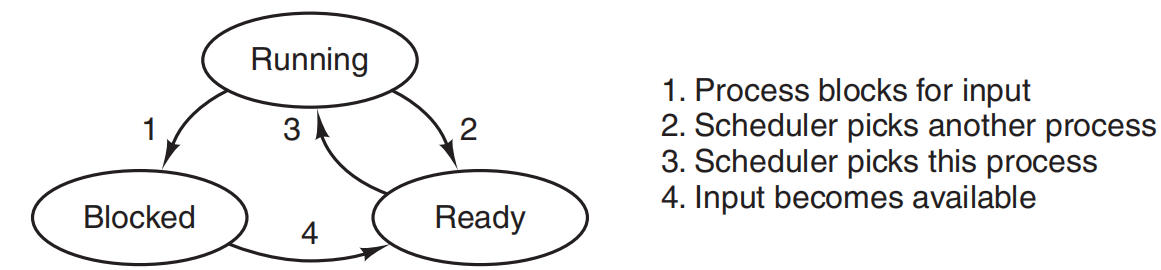
\includegraphics[width=0.85\textwidth]{FIG/2-2.png}
		\caption{一个进程有运行,就绪和阻塞三种状态,该图展示了进程如何在这三种状态下转换} \label{fig:processstatus}
	\end{figure}

	在这三种状态中,有四种转换方式。当操作系统发现一个进程不能立即继续的时候发生转换1。进程有时候可以执行一个系统调用如Pause,来进入阻塞状态。在其他的系统中,包括UNIX,当一个进程从一个管道或特殊文件中读取数据的时候,而且那时还没有可用的输入,则该线程自动进入阻塞状态。迁移3发生在所有其他进程都有了公平的份额,并且是第一个进程让CPU再次运行的时候了。调度的主题,即决定哪个进程应该运行什么时候、多长时间,是一个重要的问题;我们将在本章后面讨论它。许多算法被设计用来平衡系统的整体完全需求,以及保证对每一个进程的公平性。我们将在本书的稍后谈论到这些。迁移4发生在一个进程等待外部事件发生的时候。如果没有其他的线程在那时运行,则过程3将被触发,进程将开始运行。否则,它将需要在就绪状态进行一会等待,直到CPU可以用了才轮到它。
	使用这个进程模型,思考系统内部发生的事情变得容易得多。一些进程执行用户键入的命令程序,还有一些进程是系统的一部分,它们处理像文件服务的请求,管理运行一个磁盘或者一个磁带的具体细节。当一个磁盘中断出现的时候,系统决定停止运行现有的进程并运行磁盘进程,该进程因为之前等待中断而处于阻塞状态。因此,就可以不再考虑中断,而只是考虑用户进程,磁盘进程和终端进程等等,当他们在等待一些事情发生的时候。当磁盘被读取或者字符被键入的时候,等待它的进程已经解除阻塞,可以再次运行了。
	
	这个视图产生了图 \ref{fig:scheduler} 所示的模型。这里操作系统中最底层级的是调度器,它的上面是一系列的进程。所有的中断处理和实际运行和停止进程的细节都隐藏在调度器的里面了,调度器的实际上代码不多。操作系统的其余部分在流程形式上结构良好,然而,很少有真正的系统像这样结构良好。 

	\begin{figure}[ht]\small
		\centering
		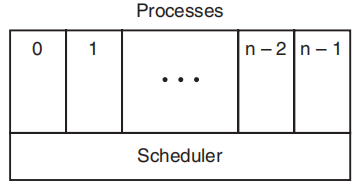
\includegraphics[width=0.85\textwidth]{FIG/2-3.png}
		\caption{最底层基于进程的操作系统处理中断和调度,在此层之上是顺序进程} \label{fig:scheduler}
	\end{figure}

	\subsection{进程实现}
	
	为了实现进程模型,操作系统维护一个表,称为进程表(一个数组结构),每一个进程有一个进程表项,一些作者称这些表项为进程控制块(PCB)。这个表项包含进程状态的重要信息,包括它的程序计数器,栈指针,内存分配地址,所打开文件的状态,它的计数与调度信息,以及进程当进程从运行态切换到就绪态和阻塞态时,必须保存的其他内容,这样它可以在稍后重新启动,就好像从未被停止过一样。
	
	图 \ref{fig:processentry} 给出了一个典型系统的关键字段,第一列中的字段关于进程管理,另外两个分别是关于内存管理和文件管理的。值得注意的是进程包含的字段是和具体的系统强关联的,各个系统可能会有很大的不同,但是该图给出了所需要信息类别的基本情况。

	\begin{figure}[ht]\small
		\centering
		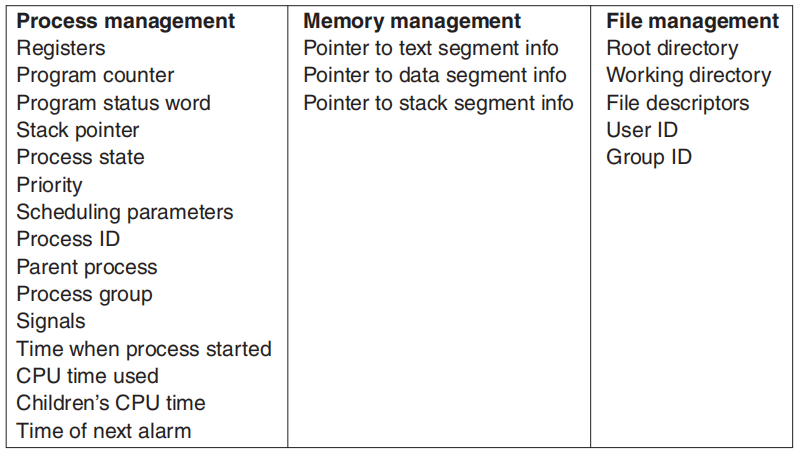
\includegraphics[width=0.85\textwidth]{FIG/2-4.png}
		\caption{一个典型的进程表项的字段} \label{fig:processentry}
	\end{figure}

	现在我们来看一下进程表,现在可以稍微多解释一些多个顺序进程是如何在一个CPU上进行管理的。和每一个I/O类别相关的是一个叫做中断向量(interrupt vector)的位置(通常位于内存底部空间的一个固定位置),它包含了中断服务过程的地址。想象一下,在用户进程3运行的时候一个磁盘中断发生了。用户进程3的程序计数器,程序状态字,有时候还有一个或多个寄存器被中断控制硬件压入到当前栈中。计算机接着就跳入到中断向量的特定地址上了,这些都是硬件所做的。从现在开始,主要就依赖软件了,特别是中断服务过程。
	所有的中断通过保存寄存器开始的,通常在当前进程的进程表条目中。接着被中断压入栈的信息被移除而且栈指针被设置指向一个暂时的栈
	进程处理器。
	像保存寄存器和保存栈指针等操作,甚至不能使用像C语言一样的高级语言进行表达,所以它们使用汇编语言的一个例程进行表达。通常对于所有的中断该例程都是可用的,因为保存寄存器的功能是可用的,不管引起中断的原因是什么。
	当这个例程结束的时候,它调用一个C过程来处理某个中断类型剩下的工作(我们假定操作系统是用C语言编写的,通常实际的操作系统都是用C语言编写的)。当完成这些工作后,一些进程可能就处于就绪状态了,调度器被调用来决定哪一个进程接下来被运行。
	中断处理和调度如图 \ref{fig:interupt} 所示。值得注意的是,细节随着系统的不同有可能会有所不同。

	\begin{figure}[ht]\small
		\centering
		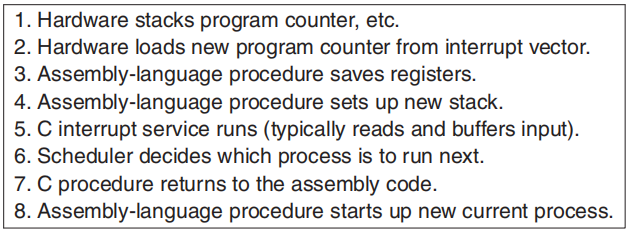
\includegraphics[width=0.85\textwidth]{FIG/2-5.png}
		\caption{中断发生后操作系统最底层的工作步骤} \label{fig:interupt}
	\end{figure}
	
	另外一个更好的模型是从概率的角度来考察CPU的利用率。假设一个进程在等待I/O完成时花费了它的一小部分时间。如果在内存中有n个进程,n个进程都在等待I/O的概率是p$^{n}$。CPU的利用率可以使用公式: \begin{center} CPU利用率 = 1 − p$^{n}$ \end{center} 表示。
	
	图 \ref{fig:multiprogrammingdegree} 给出了CPU的占用率是n的函数,我们称为多道程序设计的道数。
	
	\begin{figure}[ht]\small
		\centering
		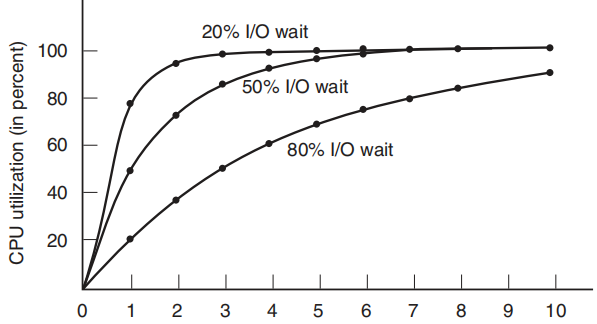
\includegraphics[width=0.85\textwidth]{FIG/2-6.png}
		\caption{CPU的利用率是内存中进程数目的函数} \label{fig:multiprogrammingdegree}
	\end{figure}

	从图中我们可以看到,进程在使用80\%的时间在等待I/O。至少有10个进程同时驻留在内存中以使得CPU的空闲率低于10\%。当您意识到等待用户在终端输入内容(或单击图标)的交互进程处于I/O等待状态时,应该很清楚,80\%或更多的I/O等待时间并不罕见。但是,即使在服务器上,执行大量磁盘I/O的进程通常也会有这个百分比或更多。
		
	为了准确起见,应该指出的是概率模型描述的只是一个估计的值。它隐式地假设所有n个进程都是独立的,这意味着内存中有五个进程的系统,其中有三个进程在运行,两个进程在等待是可以接受的。但是对于只有一个CPU,我们是不能同时运行三个进程的,因此,一个进程在CPU繁忙时准备就绪就必须等待。因此,这些过程不是独立的。可以使用队列理论建立一个更精确的模型,但是,我们所做的多道程序设计的要点是,让进程在CPU空闲时使用它,当然,仍然有效,即使的真实曲线与图中所示的曲线略有不同。尽管图 \ref{fig:multiprogrammingdegree} 所表示的模型思想简单,但是它仍然可以对CPU的性能进行特定的预测,尽管只是粗略地预测。
	假设,例如,一台计算机有8GB的内存,操作系统及其表占用2GB,每个用户程序也占用2GB。这个大小就允许有三个用户程序同时在内存中。对于平均80\%的I/O等待,我们有CPU的平均利用率(忽略操作系统的开销)为 1-0.8$^{3}$ 49\%。再增加8GB的内存可以使得系统从3道多道程序编程到7道多道程序编程,因此可以将CPU的利用率提升至79\%。换句话说,额外增加8GB内存可以使得吞吐率提升30\%。
	当然,再增加8GB内存只能使得CPU的利用率从79\%增加到91\%,仅仅只是增加了12\%的吞吐率。使用这个模型,计算机的拥有者可以判断出来,第一次增加内存的投资是划算的,而第二次增加内存的投资就不那么值得了。
	
	\section{线程}
	
	在传统的操作系统中,每一个进程都有一个地址空间和一个单个的控制线程。事实上,这几乎是进程的定义。不管怎么说,在很多的情况下,总是希望多个控制线程在同样的地址空间并以准并行化的方式处理,就好像他们是独立的进程一样(除了共享地址空间)。在接下来的章节中我们将这些情况和他们的影响。
	
	\subsection{线程的使用}
	
	为什么人们在进程内部还要有一个进程? 有若干理由说明产生这些迷你进程(线程)的重要性。现在让我们探讨一下其中的一些原因。有线程的主要原因是在许多的应用程序中,会同时发生多种活动,一些可能随着时间的推移被阻塞。通过将这些应用程序分解成多个可以准并行运行的顺序线程,可以使程序设计模型变得简单。
	
	前面已经进行了有关的讨论。准确地说,这正是之前关于进程模型的讨论。除了考虑中断,定时器和上下文切换,我们还可以考虑并行进程。
	只是现在对于线程我们增加了一个新的元素:并行的实体共享一个地址空间,并且在它们之间共享数据。这个能力对于一些应用程序而言非常地关键,而这正是多进程模型(它们具有不同的地址空间)所无法表达的。
	
	第二个需要多线程的理由是,因为线程比进程更加轻量级,它们比进程更加容易被创建和销毁。在许多系统中,创建一个线程通常比创建一个进程要快10-100倍。当线程的数量需要动态和快速地变化时,这个性质就非常地有用。
	
	使用线程的第三个原因涉及性能方面的考量。当所有线程都是CPU密集型的是时候,它们不会产生性能提升,但是如果线程既有顺序计算又有顺序I/O的时候,线程允许这些活动的重叠,从而可以提升这些应用程序的性能。
	
	做后,线程在拥有多个CPU的系统上是很有用的,因为可以实现真正的并行。我们将在第8章回过头来讨论这个问题。
	
	通过查看一些具体的示例,可以很容易地看出线程为什么有用。我们先考虑第一个例子,一个文字处理软件。文字处理程序通常在屏幕上显示正在创建的文档,因为它在屏幕上精确地显示文档。特别地,所有的换行和换页都在他们正确和最终的位置上。以便用户可以检查它们,并在需要时更改文档(比如,消除孤行,在一页上的不完整的底部行或者顶部行,因为它们看起来不够美观。)
	设想用户正在写一本书,从作者的角度看,把一本书的作为一个单独的文档,进行全书查找和全局替换的时候是最方便的。另一种方法是,每一章作为一个独立的文件。但是,把每一节和每一小节作为一个独立的文件,在进行全局替换的时候就会变得非常麻烦,因为它们可能要对上百个文件逐一进行编辑。例如,如果"某某标准草案"在书籍出版发行之前被批准了,则必须将"某某标准草案"改为"某某标准"。如果整本书只有一个文件,那么只要对一个文件进行替换处理就可以了,但是如果整本书被分成了几百个文件,则就要一个一个地对其进行修改。
	
	现在考虑,如果现在用户在一个有800页的书籍的第一页上删除一个语句,会发生什么情形。在检查了所修改的页面并确认正确以后,他想在第600页再做一次修改,并且键入一个命令告诉文字处理程序跳转到第600页(可能要查阅只是出现在那里的一个短语)。于是,字处理软件就需要对整本书的前600页进行重新排版,因为在它重新处理完前600页之前,它不知道第600页现在第一行的内容是什么。而在第600页的页面真正在屏幕上显示出来之前,计算机可能需要出现一定的延迟,这将导致用户的体验变差。
	
	多线程可以在这个时候发挥作用。想象一下文字处理软件被写成了一个两个线程的程序。一个线程用于前台和用户交互,另一个线程在后台处理重新排版。一旦第一页的一句被删除掉,交互线程立即通知排版线程立即对全书进行重新地排版。于此同时,交互线程继续监听键盘和鼠标,并响应一些简单的用户操作,如滚动页面1,而另一个线程在正后台疯狂地执行运算。幸运的是,重现排版可以在用户要求跳转到第600页之前完成,这样就可以直接显示第600页给用户了。
	
	既然做到了这个地步,那为什么不增加第三个线程呢。很多的文字处理软件都有每隔几分钟自动地保存真个文件到磁盘上的功能,防止用户在程序崩溃,系统崩溃和断电的情况下丢失掉一整天的工作。第三个线程就可以处理磁盘备份,而不对另外两个线程产生干扰。图 \ref{fig:multithreads} 给出了有三个线程的情形。

	\begin{figure}[ht]\small
		\centering
		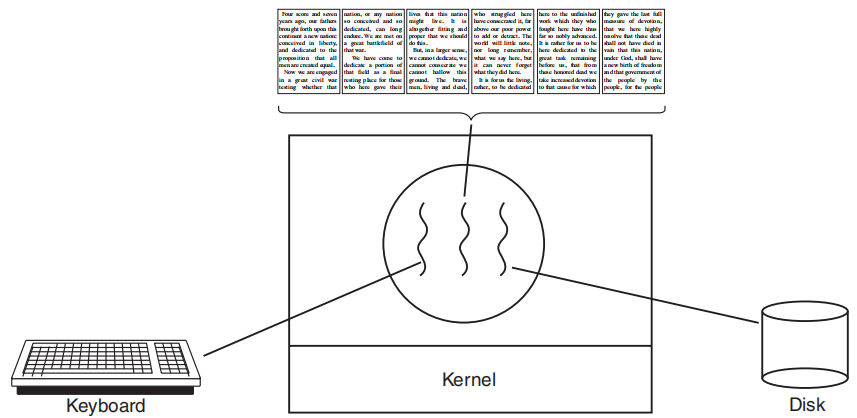
\includegraphics[width=0.85\textwidth]{FIG/2-7.png}
		\caption{一个拥有三个线程的文字处理软件} \label{fig:multithreads}
	\end{figure}
	
	如果一个程序是单线程的,那么不管什么时候开始进行磁盘备份,来自键盘和鼠标的命令在备份完成之前都将被忽视。用户当然会认为这样性能是很差的。另外,键盘和鼠标事件可以中断磁盘备份,可以实现好的性能,但是将会导致一个复杂的中断驱动编程模型。有了三个线程,编程模型就变得简单多了。第一个线程和用户进行交互,第二个线程对文档进行处理,第三个线程负责定时将RAM中的内存往磁盘备份。
	
	很清楚的是,如果有三个进程则不会这样,因为三个线程都需要操作文档。通过三个线程而不是三个进程,线程间可以共享同一块内存,因此都可以访问正在被编辑的文档,而三个进程则不可能做到这样。
	
	许多交互式程序都有类似的情形。例如,一个电子的表格允许用户维护一个矩阵,它的一些元素是用户提供的数据,另外一些元素是基于用户输入的数据采用可能比较复杂的公式计算出来的数据。当用户更改一个元素时,可能需要重新计算很多其他的元素。有一个后台线程进行这些计算,交互线程可以让用户在后台执行计算的时候进行额外的改变。类似地,第三个线程可以定期地执行磁盘备份。
	
	现在考虑线程有用的另外一个例子:一个网站的服务器。对于页面的请求进入,同时被请求的页面返回给客户端。在大多数的网站中,有一些网页的访问频率远远高于其他网页。例如,Sony主页的访问频率要远远高于深藏在页面树里的任何一款照相机的技术说明网页。网络服务器利用这个事实来将一些经常被访问的网页放到内存中,消除了需要去磁盘上取出它们的必要。像这样的集合被称为缓存,也在许多其他的场景中得到应用。我们已经在第一章中讨论了CPU的缓存。
	
	一种组织网络服务器的方式如图 \ref{fig:multithreadswebserver} 所示。这里有一个派发器线程,读取来自网络的请求。在检查完请求后,它选择一个空闲的工作线程来处理这个请求,可能是通过将一个指向消息的指针写入与每一个线程特定的字里。分派器唤醒睡眠工作线程,并将它从阻塞状态移到就绪状态。
	
	\begin{figure}[ht]\small
		\centering
		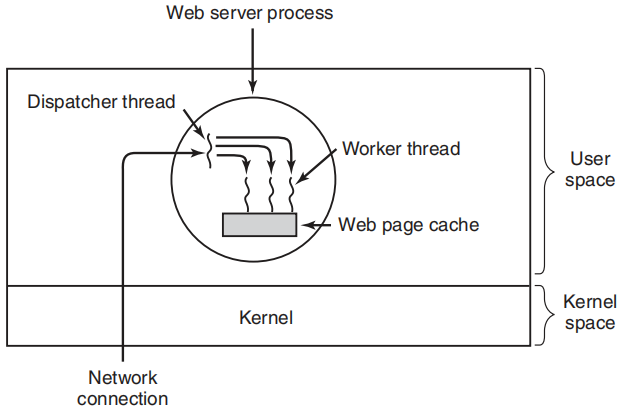
\includegraphics[width=0.85\textwidth]{FIG/2-8.png}
		\caption{一个多线程的网络服务器} \label{fig:multithreadswebserver}
	\end{figure}

	当工作进程唤醒的时候,它检查该网页请求可以从所有线程都可以访问的网页缓存中找到。如果不能找到,则开始一个\texttt{read}操作,从磁盘中读取该网页,并且阻塞该线程直到磁盘操作结束。
	
	当线程在磁盘操作上阻塞的时候,另外一个线程将被选择运行,可能是分派器,以获取更多的工作,或者是另外一个已经就绪的工作线程。
	
	这个模型使得服务器可以被写成一组顺序线程。分派器程序包括一个无限循环以获得工作请求,并把它交给工作线程。每一个工作线程的代码都有一个无限循环来接收来自分派器的请求和检查所请求的网页是否在网页缓存中。如果在,就把它返回给客户端,然后工作线程阻塞直到新的请求到来。如果不在,则从磁盘中获取该网页,并返回给客户端,接着阻塞等待一个新的请求。
	
	图 \ref{fig:coderouting} 给出了有关代码的大致框架。在这里,还有本书剩余的部分,\texttt{TRUE}被设定为常量1。同样,\texttt{buf}和\texttt{page}分别保存工作请求和网页的相应结构。
	
	\begin{figure}[ht]\small
		\centering
		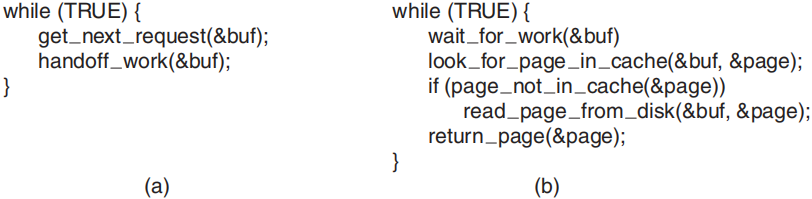
\includegraphics[width=0.85\textwidth]{FIG/2-9.png}
		\caption{图2-8的代码架构 (a)分派器线程 (b)工作线程} \label{fig:coderouting}
	\end{figure}
	
	考虑一下没有线程网页服务器该如何实现。一种可能是让他作为一种可以操作的单个线程。网页服务器使用一个主循环获得请求,检查它,并在下一个请求到来之前把它执行完毕。当等待磁盘的时候,服务器是空闲的并且不处理其他任何到来的请求。如果网页服务器运行在一个特定的机器上,而且这是通常的情况,当网页服务器在等待磁盘的时候CPU就是简单的空闲。结果就是每秒只有很少的线程被处理,所以,线程很好地改善了性能,而且每个线程通常是按照顺序编程的。
	
	目前为止,我们看到了两种可能的设计:一个多线程的网络服务器和一个单线程的网络服务器。假设一下多线程如果不可行,而系统设计者发现由于单线程带来的性能损失是不可以接受的。如果一个不阻塞的\texttt{read}系统调用是可用的,则还可以有第三种方法。当一个请求来的时候,唯一的线程就会检测到它。如果它可以从缓存中得到满足,则很好,如果不能,一个非阻塞的磁盘操作就开始了。
	
	服务器在一个表格中记录下当前请求的状态,接着去取下一个事件。下一个事件可能是一个新工作的请求也可能是前一个操作从磁盘返回的回应。如果是新的工作,则开始工作。如果是从磁盘返回的回复,将会从表格返回相关的信息,并处理回复。对于不阻塞的磁盘I/O,回复可能需要以信号或者中断的形式返回。
	
	在这个设计中,我们在头两个模型中的“顺序进程”模型消失了。计算的状态每次都必须显式地保存在表中,当服务器从一个请求切换到另外一个请求的时候。事实上,我们在以一种非常硬核的方式模拟线程和它的栈。一种像这样的设计,在其中每一个计算都有保存的状态,而且存在一些事件可以出现来改变这种状态,被称为“有限状态机”。这个概念在计算机科学中被广泛地应用着。
	
	现在对于线程应该提供什么就已经非常清楚了。它们使我们能够保留顺序进程的思想,即进行阻塞调用(例如,对于磁盘I/O),并且仍然能够实现并行性。阻塞系统调用可以使得编程变得简单,而且并行性可以改善性能。单线程的服务器保持了阻塞系统调用的简单性但是放弃了性能。第三种方法通过并行性取得了高的性能但是使用了非阻塞的调用和中断,因而很难编程。这些模型的优缺点都在图 \ref{fig:threeways} 中所示了出来。
	
	\begin{figure}[ht]\small
		\centering
		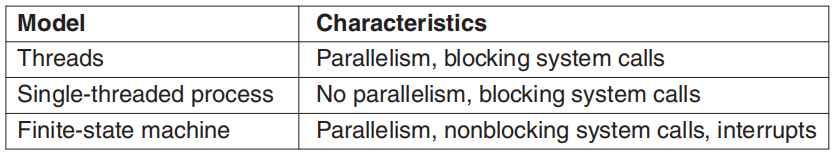
\includegraphics[width=0.85\textwidth]{FIG/2-10.png}
		\caption{构建服务器的三种方式} \label{fig:threeways}
	\end{figure}
	
	第三个关于进程作用的例子是那些必须处理极大数量数据的应用。通常的方式是读入一个数据块,处理它,并把它写出。这里的问题是如果仅仅只能用阻塞的系统调用,进程在数据输入或输出的时候就会被阻塞。在需要有大量的计算的时候,使得CPU空闲,无疑是浪费的,应该尽量避免。
	
	多线程提供了一种解决方案。进程可以被分解成一个输入线程,一个处理线程和一个输出线程。输入线程读入数据到一个缓冲区中,处理线程从缓冲区中取出数据,处理它们,并把结果放置到一个输出缓冲区中。输出缓冲区将这些结果写回到磁盘。在这种方式下,输入,输出和处理可以同时进行。当然,这个模型仅仅在系统调用只阻塞调用线程的时候才有用,而不是阻塞整个进程。
	
	\subsection{经典的线程模型}
	
	现在我们已经看到为什么线程是有用的而且它是如何被使用的,让我们更多地调查一下这个想法。进程模型基于两个基本的概念:资源分组和执行。有时候很难去区分它们,这就引入了线程的概念。首先,我们看一下经典的线程模型,接着我们将看一下Linux的进程模型,它模糊了进程与线程的分界线。
	
	理解进程的一个视角是,它是一个组织相关资源在一起的方式。一个进程有一个包含程序文本和数据的地址空间,同样也有其他的资源。这些资源可能包括打开的文件,子进程,即将发生的定时器,信号处理程序,账户信息等等。把它们以进程的形式放在一起,可以更好地进行管理。
	
	进程的另外一个概念是一个正在运行的线程,通常被简称为线程。这个线程有一个程序计数器来跟踪接下来执行哪一条指令。它有寄存器,来保存现有的工作变量。它有一个栈,来包含执行历史,每一个过程都有一帧,但是尚未返回的帧。尽管一个线程必须在一些进程中执行,线程和进程是不同的概念,可以分别给予处理。进程可以被用来组织资源,线程是在CPU上被调度的执行实体。
	
	线程给进程模型带来的丰富是允许多个执行操作在一个相同的进程环境中发生,允许彼此之间有较大独立性的多个线程执行。在一个进程有多个线程并行执行类似于在一台计算机中有多个进程并行执行。在前一个情况下,线程之间共享地址空间和其他的资源,在第二种情况下,进程共享物理内存,磁盘,打印机和其他资源。因为线程有一些进程的性质,它们有时候又被称为轻量级线程。术语"多线程"也被用来描述在一个进程中有多个线程的情况。就像我们在第一章中看到的那样,一些CPU有一些对多线程的直接硬件支持,并且允许线程在纳秒级时间内进行切换。
	
	在图 \ref{fig:processthread} (a)中我们看到三个传统的进程。每一个进程都有它的地址空间和单个控制线程。相反,在图 \ref{fig:processthread} (b)中我们看到一个进程有三个控制线程。尽管两种情况下我们都有三个线程,在图 \ref{fig:processthread} (a)每一个进程都操作在一个不同的地址空间上,而在图 \ref{fig:processthread} (b)中三个进程共享同一个地址空间。
	
	\begin{figure}[ht]\small
		\centering
		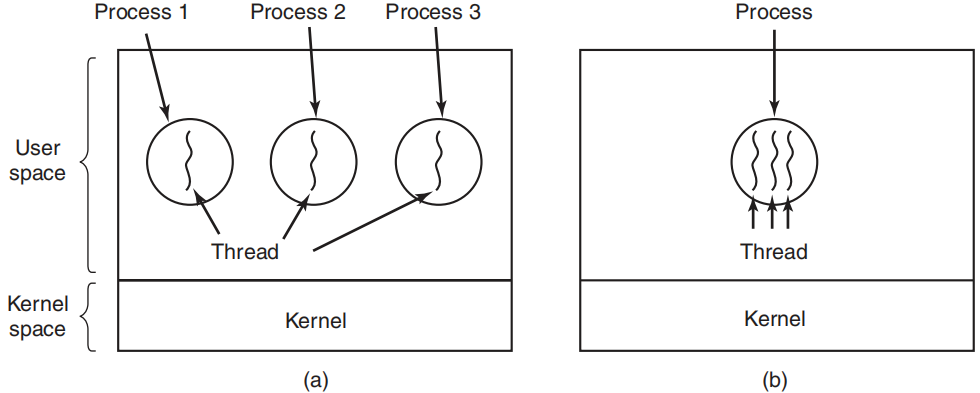
\includegraphics[width=0.85\textwidth]{FIG/2-11.png}
		\caption{a)三个进程每个含有一个线程,b)一个进程包含三个线程。} \label{fig:processthread}
	\end{figure}

	当一个多线程的进程运行在一个单CPU的系统上时,线程轮流被执行。图 \ref{fig:processconcept} 给出了一个多道编程的进程是如何工作的。通过在多个进程之间来回地切换,系统给出了多个顺序进程是并行执行的假象,多线程也是这样工作的。CPU在多个线程之间来回地切换,提供了多个线程也是并行执行的假象,好像它们运行在比实际CPU更慢一些的CPU上。在一个有三个计算密集型的线程的进程中,线程可以表现出并行的性质,每一个线程得到真实CPU速度的三分之一。
	
	一个进程中的不同线程不像不同的进程那样地相互独立性。所有的线程都有相同的地址空间,同时也意味着它们共享相同的全局变量。因为每个线程都可以访问进程地址空间的每一个内存地址,一个线程可以读,写甚至清空另一个线程的栈。线程之间没有保护,因为: 1)不可能, 2)也不必要。和不同的进程不同,可能来自不同的用户,而且彼此之间可能还有敌意,一个进程总是被单个用户所拥有,它们大概总会创建多个线程,线程之间是相互合作而不是斗争。除了共享地址空间,所有的线程还可以共享打开的文件集,子进程,时钟,信号等等。像图 \ref{fig:sharecontents} 所示的那样。

	\begin{figure}[ht]\small
		\centering
		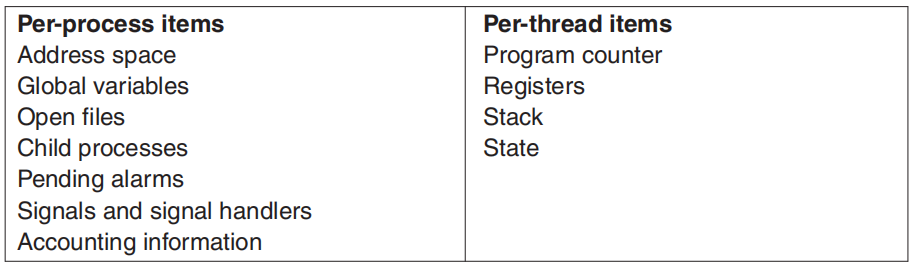
\includegraphics[width=0.85\textwidth]{FIG/2-12.png}
		\caption{a)第一列给出了线程间共享内容 b)第二列给出了线程间私有内容} \label{fig:sharecontents}
	\end{figure}
	
	第一列中的项目是进程属性,不是线程属性。例如,如果一个线程打开了文件,这个文件对于进程中的其他线程也是可见的,它们可以进行读和写。这是合理的,因为进程是进行资源管理的单元,不是线程。如果每一个线程都有它的地址空间,打开的文件,挂起的时钟等等,它将会是一个独立的进程。我们努力通过线程的概念来使得多个线程可以执行来获取一组资源这样它们就可以一起紧密地合作来完成工作任务。
	
	像一个传统的进程(一个进程仅仅只有一个线程),一个线程只能是以下几种状态的一种:运行,阻塞,就绪或终止。一个运行的线程当下拥有CPU并且是活动的。相比较而言,一个阻塞的线程等待一些将它解除阻塞的事件发生。例如,当一个线程执行一个系统调用从键盘读取数据的时候,该线程就被阻塞直到输入被键入。一个线程可以处于阻塞状态直到一些外部的事件发生,或者等待其他的线程来解阻塞它。一个就绪的线程将被安排运行,而且一到轮到他就会被运行。线程之间的状态转换和进程之间的状态转换是一样的,如图 \ref{fig:processstatus} 所示。
	
	意识到每一个进程都有自己的堆栈是非常重要的,像图 \ref{fig:threadstack} 中所示的那样。每个线程的堆栈包含一个帧,用于调用的每个过程但是尚未从返回。
	
	\begin{figure}[ht]\small
		\centering
		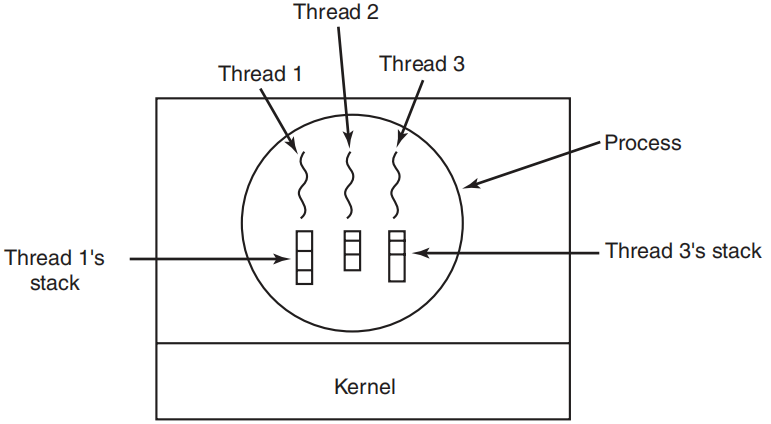
\includegraphics[width=0.85\textwidth]{FIG/2-13.png}
		\caption{每一个线程都有自己的栈} \label{fig:threadstack}
	\end{figure}

	这个帧包含过程的局部变量和过程调用结束后的返回地址。例如,如果过程X调用过程Y,过程Y调用过程Z,而过程Z正在被执行。则过程X,Y和Z的帧都将在栈上。每一个线程都会调用不同的过程并且都有一个不同的执行历史。这就是为什么每一个线程需要它自己的栈的原因。
	
	当多线程存在的时候,进程可能会从一个单线程开始。线程拥有创建新线程的能力通过调用库过程,如\texttt{thread\_create}。
	一个\texttt{thread\_create}的参数指定新线程运行过程的名字。没有必要指定新线程的地址空间,因为新线程会在创建线程的地址空间中自动运行。一些线程是有层次的,有父子关系,但是这种关系并不常见,大部分情况下线程之间是平等的。无论有没有层次关系,创建的线程都会返回一个标识符,该标识符也就是新线程的名字。
	
	当一个线程终止了它的工作,它可以通过调用一个库过程退出,称为\texttt{thread\_exit},接着它就消失了并且不会被调度了。在一些线程系统中,一个线程可以通过调用一个过程来等待另外一个线程退出,例如\texttt{thread\_join}。这个过程阻塞调用它的线程直到另一个线程退出。在这一点上,线程的创建和终止非常类似于进程的创建和终止,也有大致相同的选择。
	
	另外一个常见的线程调用是\texttt{thread\_yield},允许一个线程主动地放弃CPU并让另外一个线程运行。这样的调用很重要,因为没有时钟中断可以像进程那样实际执行多道程序设计。因此,线程非常友善地主动放弃CPU让其他线程运行是非常重要的。有的调用允许一个线程等待另一个线程完成它的工作,或让一个线程宣称它已经完成了一些工作,等等。
	
	虽然线程很有用,但是它们也同时给编程模型带来了许多其他的复杂性。一开始,考虑一下UNIX中的系统调用。如果父进程中有多个线程,那么子进程中是不是也应该有多个线程呢? 如果不是,则进程可能不能正常地工作,因为在该子进程中的线程都是绝对必要的。
	
	然而,如果一个子进程像父进程一样拥有同样多的线程,如果父线程在读调用(例如,从键盘)被阻止,会发生什么情况? 那是不是两个线程被阻塞到键盘上了,一个是父进程,一个是子进程? 当键入一行命令的时候,是不是两个线程同时获得了相应的副本? 还是仅仅是父进程,仅仅是子进程。
	
	另外一类问题是关乎线程共享许多数据结构的事实。当一个线程关闭一个文件而另一个线程还在读取它的时候会发生什么。假设一个线程发现内存太少而开始分配更多的内存。在工作一半的时候,发生了进程切换,新的线程同时也注意到了内存太少并开始分配更多的内存。内存有可能被分配两次,这个问题可以通过一些努力给解决,但是需要仔细的思考和设计才能使多线程程序能够正确地工作。
	
	\subsection{POSIX进程}
	
	为了实现可移植的线程程序,IEEE制定了一个关于线程的标准: IEEE 1003.1c。它定义的线程包被称为Pthreads。大部分UNIX的系统支持它。这个标准定义了超过60个函数调用,太多了不能一一列举。这里我们只列举几个主要的来说明它是怎么工作的。
		
	\begin{figure}[ht]\small
		\centering
		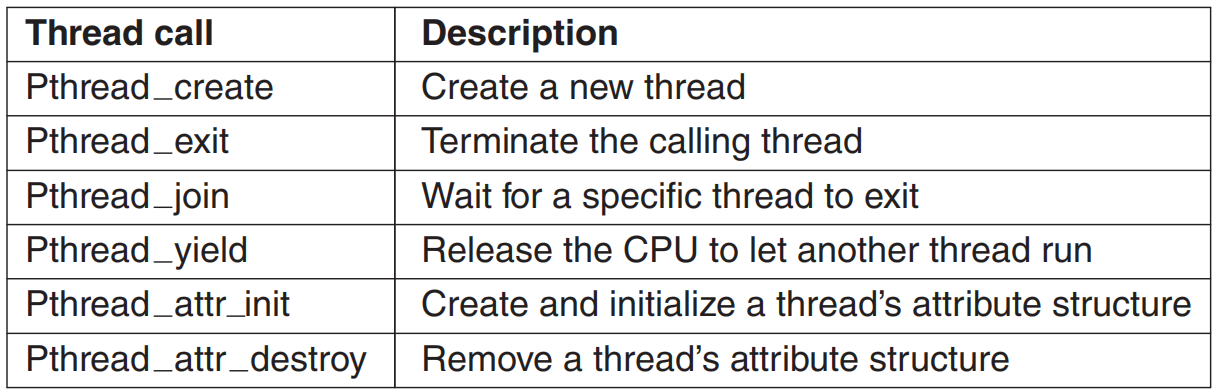
\includegraphics[width=0.85\textwidth]{FIG/2-14.png}
		\caption{一些Pthread函数调用} \label{fig:pthread}
	\end{figure}

	所有的Pthreads线程都有特定的性质。每一个都有一个标识符,一组寄存器(包括程序计数器)和一组属性,被存储在一个结构中。这些属性包括栈大小,调度参数,还有一些其他使用线程所需要的项目。
	
	一个新线程的创建使用\texttt{pthread\_create}调用。新创建线程的线程标识符作为函数返回值使用。这个调用非常类似与fork系统调用(除了参数),线程标识符扮演着PID的角色,主要用于识别其他调用中引用的线程。
	
	当一个线程已经完成了分配给它的工作,它可以调用\texttt{pthread\_exit}终止。这个调用中止线程并释放它的栈。
	
	一般一个线程在继续需要等待另外一个线程完成它的工作并退出。等待的线程调用\texttt{pthread\_join}来等待另一个特定的线程终止。被等待线程的线程标识符被当作参数传递。有些时候碰巧有些线程逻辑上没有被阻塞,但是感觉它已经运行了很长的时间,并且想给另外一个线程运行的机会。它可以通过\texttt{pthread\_yield}系统调用来实现。对于进程则没有这样的假设,因为我们假设进程之间是激烈竞争的,每一个进程都想获得所有的CPU时间。然而,因为一个进程中的所有的线程都是在一起工作的,它们的代码也大部分是一个人写的,有时候编程者希望这些线程互相能给对方一个机会。
	
	接下来的两个系统调用,处理属性。\texttt{Pthread\_attr\_init}创建和一个线程相关的属性结构,并把它们初始化为默认值。这些值(如优先级)可以通过操作属性结构中的字段来进行改变。
	
	最后,\texttt{Pthread\_attr\_destory}移除一个进程的属性结构,释放它的内存。它不会影响调用它的线程,调用它的线程会继续存在。
	
	为了更好地体验Pthreads是如何工作的,考虑一下图 \ref{fig:threadexample} 所示的简单例子。
	
	\begin{figure}[ht]\small
		\centering
		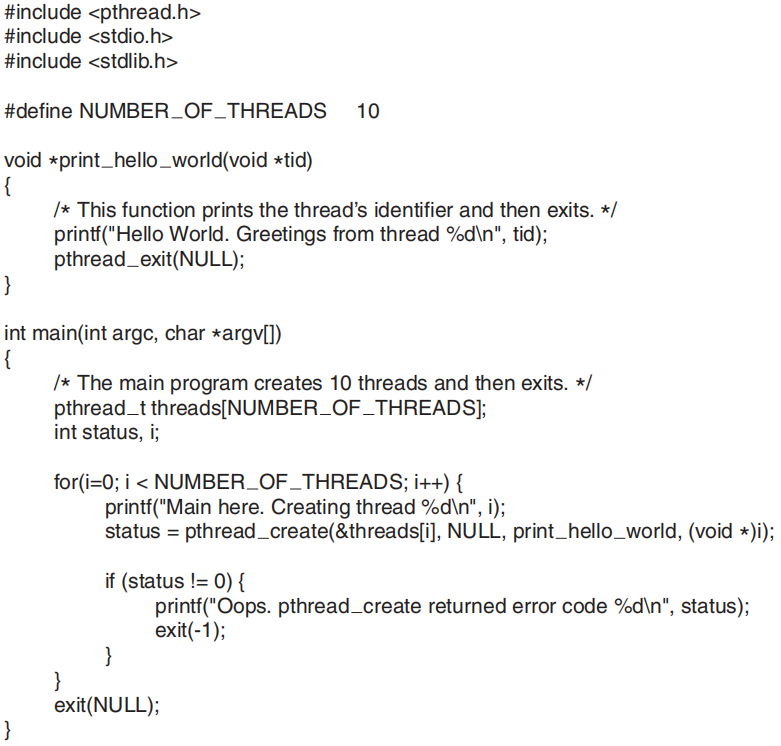
\includegraphics[width=0.85\textwidth]{FIG/2-15.png}
		\caption{一个使用线程的示例程序} \label{fig:threadexample}
	\end{figure}
	
	这里主程序循环了\texttt{NUMBER\_OF\_THREADS}次,在每一次的迭代中创建一个新的线程,在声称了它的打算之后。如果线程创建失败了,它打印一个错误信息并退出。在创建了所有的线程后,主程序退出。
	
	当一个线程被创建后,它打印一个一行的程序来声称它自己,接着就退出。各种信息交织的顺序是不确定的,在程序运行时可能会有所不同。
	以上谈论的Pthread调用不是全部的,我们将看一下其他的系统调用在讲述完进程和线程同步后。
	
	\subsection{在用户空间实现线程}
	
	有两个主要的地方用来实现线程:用户态和内核态。这两者之间的选择稍微有些争议,有时候混合的方案也是可能的。我们将描述这些方法,以及它们0的优点和缺点。
	
	第一种方法是将整个的线程包放到用户空间中。内核不知道它的任何内容。内核关心的,是管理单线程的普通进程。首先,也是最明显的,一个用户级别线程包的好处是它可以实现在一个不支持多线程的操作系统之上。所有的操作系统都曾经属于这一类,甚至直到现在还有一些操作系统是这样的。通过这种方法,操作系统被实现成一个库。
	
	所有的这类实现都有相同的通用结构,如图 \ref{fig:threadpackage} 所示。
	
	\begin{figure}[ht]\small
		\centering
		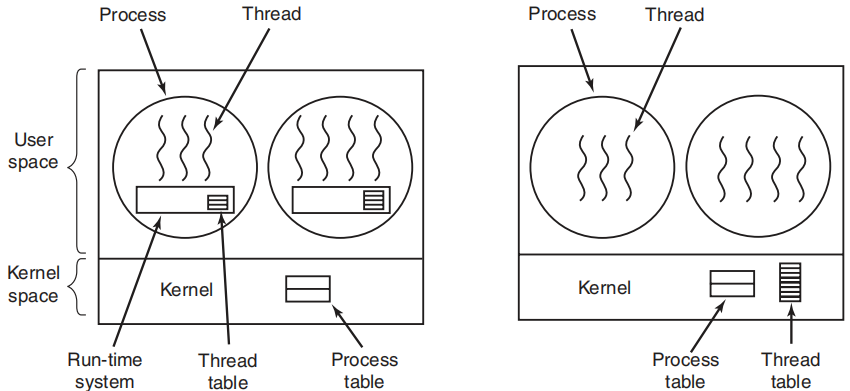
\includegraphics[width=0.85\textwidth]{FIG/2-16.png}
		\caption{(a) 一个用户级线程包 (b) 一个被内核管理的线程包} \label{fig:threadpackage}
	\end{figure}

	线程运行在运行时系统之上,运行时系统是管理线程的过程的集合。我们已经看过了四个调用: \texttt{pthread\_create}, \texttt{pthread\_exit}, \texttt{pthread\_join},和\texttt{pthread\_yield},但是通常还有更多。
	
	当线程在用户态进行管理的时候,每一个进程都需要有它私有的进程表来跟踪在进程内的线程。这个表格和内核中的进程表类似,但它只跟踪每个线程的属性,例如每个线程的程序计数器、堆栈指针、寄存器、状态等等。线程表是被运行时系统管理的。当一个线程被移至就绪态或者阻塞态,它将重启需要的信息存放到进程表格中,就像内核将进程状态存放到进程表格中是一样的。
	
	当线程做了一些可能导致它本地阻塞的操作,例如,等待线程里面的另一个线程来完成工作,它调用一个运行时过程。此过程检查线程是否必须置于阻塞状态。如果是,它存储线程的计数器(线程本身的)在线程表格中,在表中查找就绪的线程运行,并且将线程保存的值重新载入机器的寄存器中。只要线程的栈指针和程序计数器切换好,新的线程就会自动地被重新执行。如果机器正好有一个指令存储所有的寄存器以及另外一条指令把他们进行加载,则整个线程切换可以在数条指令内完成。这样进行线程切换只有比陷入内核执行切换要快一个数量级,这是使用用户级线程包一个极大的优点。
	
	但是,还有一点和进程有很大的不同。当一个线程在某一个时刻停止运行的时候,例如,它调用了\texttt{thread\_yield},\texttt{thread\_yield}的源代码可以在线程表中保存线程自身的信息。另外,它可以调用线程调度器来选择另外一个要运行的线程。保存线程状态和调度的过程都是本地过程,所以触发它们比执行一个内核系统调用要方便地多。另一方面,不需要陷入内核,不需要上下文切换,不需要刷新内存缓存等等。这些使得线程调度非常快速。
	
	用户级线程还有一些其他的优点。它们允许每一个线程都有它们自己的线程调度算法。对于一些应用程序,例如,哪些有垃圾回收器的线程,不必担心线程在一个不方便的时刻停下来是一个加分项。它们还可以扩展地更多,因为内核线程需要在内核中有一些固定的表格空间和堆栈空间,在有很多线程的时候可能会称为一个问题。
	
	尽管用户级线程包有着更好的性能,但是也有一些主要的问题。其中首要的问题是如何实现阻塞的系统调用。假设一个线程在键盘上的键被键入之前读取键盘。让这个线程真正地执行系统调用是不可接受的,因为这将阻塞其他所有的线程。使用线程的首要目标是允许每一个线程使用正在阻塞的调用,并且阻止一个阻塞线程影响到其他的线程。对于正在阻塞的系统调用,有了阻塞系统调用,这个目标不是轻易能够实现的。
	
	系统调用可以改为非阻塞的(例如,如果没有被缓冲的字符,对键盘的read操作可以只返回0字节),但是需要修改操作系统,这个方法是不具有吸引力的。除此之外,用户级线程的一个论据是它们可以执行在现有的操作系统之上。另外,修改\texttt{read}的语义需要对许多用户程序进行修改。
	
	在这个过程中,还有一种可能的替代方案,就是如果某个调用会阻塞,就提前通知。在大多数UNIX的版本中,有一个系统调用\texttt{select}可以允许调用者通知预期的\texttt{read}是否会阻塞。当出现此调用时,库过程read可以替换为一个新过程,该过程首先执行select调用,然后在安全的情况下才执行read调用(即不会阻塞)。如果\texttt{read}调用被阻塞,有关调用就不进行,代之以运行另外一个线程。到了下次有关的运行时系统获得了控制权,就再次检查运行\texttt{read}系统调用是否安全。这个过程要求重写系统调用库的一部分,效率不高也不够优雅,但是其他的选择不多。在系统调用周围从事检查的这些代码称为包装器(Jacket或者Wrapper)。
	
	与阻塞系统调用问题有点类似的是缺页中断问题。我们将在第三章中学到这个内容。此时可以认为,把计算机设置成这样的一种工作方式,如果程序调用或跳转到不在内存中的指令,则发生页错误,操作系统将从磁盘上获取丢失的指令及其相邻指令,这就称为一个缺页中断。这个进程被阻塞当必要的指令被定位和读入的时候。如果一个线程导致了一个缺页中断,则内核甚至在没有感知到线程存在的情况下,自然地阻塞整个进程直到磁盘I/O结束的时候,尽管其他的线程是可以运行的。
	
	用户级线程包的另外一个问题是,如果一个线程开始运行,其他的线程将不会被运行除非正在运行的线程主动放弃CPU。对于一个单进程而言,没有时钟中断,使得按照轮转法进行进程轮转的方法变得不可行(轮流执行)。除非某一个线程按照自己的意志进入运行时系统,否则调度器将永远不会有机会。
	
	解决线程永远运行的问题的一个可能的解决方案是运行时系统每秒请求一次时钟信号(中断)来控制它,但这对程序来说也是粗糙和混乱的。
	不可能总是发生高频率的周期性的时钟中断,即使可能,总的开销也是非常高昂的。更多的是,线程可能也需要一个时钟中断,这样就会扰乱运行时系统使用的时钟。
	
	另外,也许是对用户级线程最大的争论性意见是,程序员通常在经常发生线程阻塞的应用中才希望使用多线程。例如,在多线程Web服务器中,这些线程持续地进行系统调用,而一旦发生内核陷阱并执行系统调用,如果旧的线程被阻塞了,那么内核就不需要再做更多的工作来切换线程了,而且让内核这样做就不需要不断地进行select系统调用来检查read系统调用是否安全。对于基本上完全受CPU限制且很少阻塞的应用程序,拥有线程有什么意义? 由于这样做没有什么益处,因此没有人会用多线程来进行计算头n个素数或者下象棋之类的工作。
	
	\subsection{在内核中实现线程}
	
	现在让我们看一下内核是如何管理和实现线程的。如图 \ref{fig:threadpackage} (b)所示,此时就不再需要运行时系统了。同时,每一个进程中也没有线程表了,相反,内核中有一个追踪系统中所有线程的线程表。当一个线程想创建一个新的线程和销毁一个现有的线程,它执行一个内核系统调用,这个系统调用通过更新内核线程表来完成线程的创建和撤销工作。内核线程表持有每一个线程的寄存器,状态以及其他的信息。同时,内核还维护传统的进程表来追踪进程。所有的可以阻塞线程的调用都被实现为系统调用,一般比运行时过程有更高的代价。当一个线程阻塞的时候,内核根据其选择,可以运行该进程中的另外一个线程(如果有就绪线程)或者其他进程中的线程。对于用户级线程,运行时系统保持运行自己进程中的线程直到内核将CPU从该进程移走(或者没有就绪进程了)。
	由于内核创建和回收线程的代价相对较大,一些系统采用一种环保的方式回收其线程。当一个线程被销毁的时候,它被标记为不可以运行状态,但是它的内核中的数据结构并不受到影响。稍后,当一个线程必须被创建的时候,旧的线程重新被激活,从而节省一些开销。线程回收同样适用于用户级线程,但是由于用户级线程的管理代价要小的多,并没有很强烈的需求去这样做。
	
	内核线程并不需要任何新的,非阻塞的系统调用。另外,如果一个进程中的线程导致了一个缺页中断,内核可以很轻易地检查该进程是否还有其他可以运行的线程,如果有,则在等待从磁盘取回该页的时候运行它们其中的一个。它们的主要缺点是系统调用的代价比较大,所以如果线程的操作(创建,终止等)比较多,就会带来很大的开销。
	
	虽然内核线程可以解决一些问题,但是它不能解决所有的问题。例如,当一个多进程的线程被复制会发生什么?新的进程是不是和父进程拥有同样多的线程,还是只有一个?在大多数情况下,最好的选择取决于新的进程接下来要干什么。如果它想调用\texttt{exec}来启动一个新的程序,可能只有一个进程是正确的选择,但是如果它想继续执行,则复制所有的进程是最佳的选择。
	
	另外一个因素是信号。要记得信号是发送给进程的,而不是线程,至少在经典模式中是这样。当一个信号到来的时候,哪一个线程应该处理它?可能线程会注册它们对哪些信号感兴趣,所以当一个信号到来的时候应该交给声称对它感兴趣的线程进行处理。但是如果两个或更多的线程都注册对某一个信号感兴趣了怎么办?这仅仅是线程引发的两个问题,还有其他更多的问题。
	
	\subsection{混合实现}
	
	很多种不同的方法都被尝试用来综合用户级线程和内核级线程的优势。一种方法是使用内核级线程,然后在它们中的一些或全部复用用户级线程,像图 \ref{fig:multiplexthreads} 所示的那样。
	
	\begin{figure}[ht]\small
		\centering
		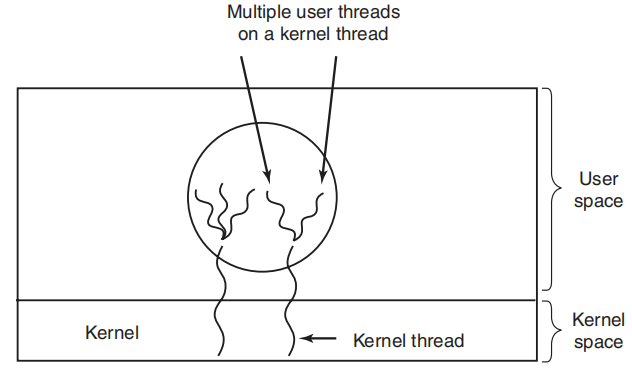
\includegraphics[width=0.85\textwidth]{FIG/2-17.png}
		\caption{将用户级线程多路复用到内核级线程} \label{fig:multiplexthreads}
	\end{figure}
	
	当采用这种方法的时候,内核可以决定使用多少内核级线程以及在每一个内核级线程上复用多少用户级线程,这种模式提供了终极的灵活性。
	在这种方法中,内核只感知内核级线程并调度它们。这些内核线程中的一些可能会在它们之上复用多个用户级线程。这些用户级线程被创建,销毁和调度,就像运行在一个不支持多线程操作系统的进程中的用户级线程一样。在这个模式中,每一个内核级线程都有轮流使用它的一组用户级线程。
	
	\subsection{调度器激活}
	
	虽然内核级线程在一些关键的方面优于用户级线程,但是它们也毫无争议地更慢。因此,研究人员一直在寻找在保留其优良特性的前提下改善其性能的方法。接下来我们将描述一个由安德森在1992年设计的一种方法,称为调度程序激活机制(scheduler activations)。其相关工作有Edler et al.(1988)和Scott et al.(1990)等。
	调度器激活的目标是模拟内核线程的功能,但是实现在用户空间中的线程包可以有更好的性能和更大的灵活性。特别地,如果用户级线程从事某种系统调用是安全的,那么它就不应该进行非阻塞的系统调用和提前进行检查。不管怎么样,当一个线程因为系统调用或缺页中断被阻塞的时候,主要在同一个进程中有任何就绪的线程,就应该有可能运行其他线程。
	
	由于避免了在用户空间和内核空间之间不必要的切换,从而提高了效率。如果一个进程阻塞等待另一个进程做一些事情的时候,例如,此时没有理由请求内核,因此节省了内核与用户空间之间的转换。用户空间的运行时系统可以阻塞同步的进程从而重新启动一个新的进程。
	
	当调度器激活机制被使用的时候,内核给每一个进程安排一定数量的虚拟处理器,并且让(用户空间)运行时系统将线程分配到处理器上。这个机制也可以被用在多处理器系统上,此时虚拟处理器可能是一个真实的CPU。分配给每一个进程的虚拟处理器的个数初始是1个,但是进程可以要求更多的虚拟处理器并在不再需要的时候将它们返回。内核还可以将已经分配出去的虚拟处理器收回以重新分配给更加需要的进程。
	
	使得这种机制工作的基本想法是当内核知道一个线程阻塞的时候(通过执行一个正在阻塞的系统调用和导致一个缺页中断),内核通知进程的运行时系统,在堆栈上作为参数传递相关线程的编号和发生的事件的描述。通知正好在内核在一个已知的地址中激活运行时系统发生了,这是对UNIX系统中一种粗略的估计,这个机制被称为上行调用(upcall)。
	
	一旦被激活,运行时系统可以重新调度它的线程,典型的是标记当前的线程为激活,并从就绪队列中取出另一个线程,设置它的寄存器,并重新启动它。稍后,当内核知道初始的进程可以再次运行(例如,它想读取的管道包含数据,引发中断的缺页已经从磁盘上取回等),内核又一次上行调用运行时系统,通知它这一事件。运行时系统可以立即重启被阻塞的线程或者将它放入就绪队列并稍后启动它。
	
	当一个用户级线程正在运行的时候出现了硬件中断,中断的CPU切换到内核态。如果中断是由于对中断不感兴趣的进程事件触发的,像另一个进程I/O的终止,当中断处理器结束的时候,它将中断线程设置回中断之前的状态。但是,如果进程对中断感兴趣,则进程的某一个线程需要的页面到达了,中断线程就没有被重启,相反,它会挂起,运行时系统会在那个虚拟CPU上启动,堆栈上中断线程的状态。接着它决定在哪一个线程调度到CPU上,是中断的那个,新就绪的那个还是第三种选择。
	
	调度激活器的另一个作用是作为上行调用的基础性依赖,这是一个违反分层次系统内在结构的概念。通常,第n层提供给第n+1层可以调用的特定服务,但是第n层不一定会调用第n+1层的过程。上行调用不遵循这个基本原则。
	
	\subsection{弹出线程}
	
	线程通常在分布式系统中被频繁地使用。一个重要的例子是如何处理传入信息,例如服务请求。传统的方法是将一个在\texttt{receive}系统调用中阻塞的进程或者线程正在等待一个到来的消息。当一个消息来临的时候,它接收这个消息,拆包它,检查它的内容并处理它。
	然而,一个完全不一样的方法也同样是可能的,其中消息的到达会导致系统创建一个新线程来处理该消息。这样的线程被称为弹出线程,如图\ref{fig:pop-upthreads} 所示。
	
	\begin{figure}[ht]\small
		\centering
		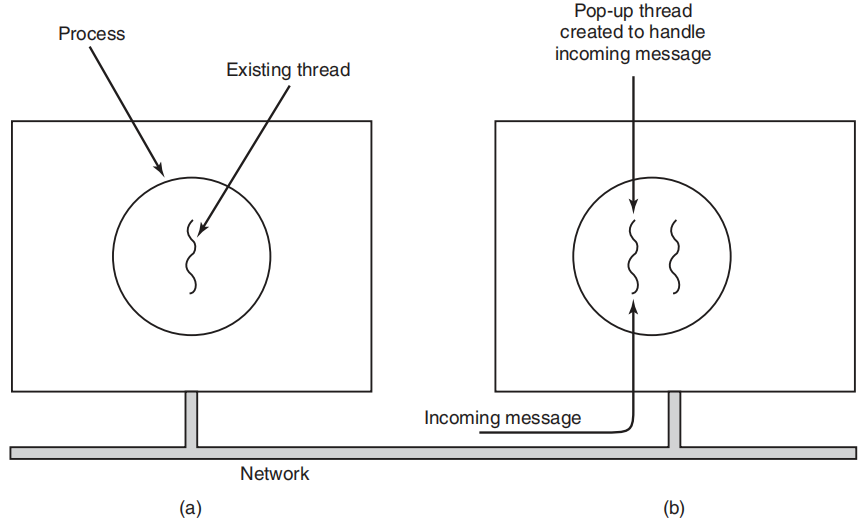
\includegraphics[width=0.85\textwidth]{FIG/2-18.png}
		\caption{当一个消息结束的时候创建新的线程。a)在消息到达之前,b)在消息到达之后。} \label{fig:pop-upthreads}
	\end{figure}

	弹出线程一个关键的好处是它们是时新的,它们没有什么历史-寄存器,栈还有它们必须存储的东西。每一个启动的线程都是新鲜的,而且每一个线程都是和其他线程类似的,这样使得快速创建一个线程称为可能,新的线程将到来的消息分配给进程。使用弹出线程的结果是使得消息到达和进程开始之间的延迟变得非常短。
	
	当使用弹出线程的时候需要做一些高级的规划。例如,在哪一个进程中运行线程?如果系统支持在内核上下文中运行线程,那么线程可能会在那里运行(这就是为什么我们没有在图 \ref{fig:pop-upthreads} 中显示内核)。在内核空间中运行线程也通常比在用户空间更加地容易和快。同样,一个内核空间中的弹出线程可以轻易地访问内核表和I/O设备,这个将有助于中断处理。另一方面,一个有错误的内核态弹出线程可以比用户态线程带来更大的危害。例如,如果它运行了太长的时间并且没有方法停止它的话,进来的数据就有可能永久地丢失了。
	
	\subsection{单线程的程序多线程化}
	
	许多现存的程序都是为单线程的进程编写的。将这些转换为多线程处理比最初看起来要复杂得多,下面我们将只讨论几个陷阱。一开始,一个线程通常包括多个过程,就像一个进程一样。它们可能会有局部变量,全局变量以及参数。局部变量和参数并不导致任何的麻烦,但是对于一个线程来说是全局的而不是整个程序的全局变量是一个问题。这些变量是全局的,意味着许多线程内的过程使用它们(只要它可能使用任何的变量),但是其他的进程在逻辑上与这些变量无关。
	
	例如,我们考虑一下UNIX维护的\texttt{errno}变量。当一个进程(或者线程)使用系统调用失败的时候,它将错误码放入\texttt{errno}中。在图 \ref{fig:globalvariableonthreads} 中,线程1执行了系统调用\texttt{access}来找出它是否有访问某一个文件的特定权限。操作系统通过\texttt{errno}错误码返回答案。
	
	\begin{figure}[ht]\small
		\centering
		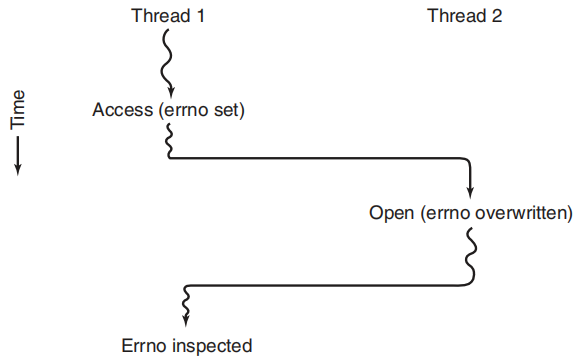
\includegraphics[width=0.85\textwidth]{FIG/2-19.png}
		\caption{进程间对于使用一个全局变量发生冲突。} \label{fig:globalvariableonthreads}
	\end{figure}

	当控制权被返回给线程1的时候,但是如果有机会读取\texttt{errno},调度器任务线程1在此时有足够的CPU时间并决定转移到线程2。
	线程2执行\texttt{Open}调用失败了,导致了\texttt{errno}被重写而线程1中的访问码永久地丢失。当线程1稍后重启的时候,它将读取到错误的值并工作错误。
	
	对这个问题可以有不同的解决方案。一个方法是禁止所有的全局变量,尽管这个方法有点不太合适,因为它同许多已有的软件相冲突。另一个解决方案是给每一个线程分配它们私有的全局变量,如图 \ref{fig:privatevariables} 所示。
	
	\begin{figure}[ht]\small
		\centering
		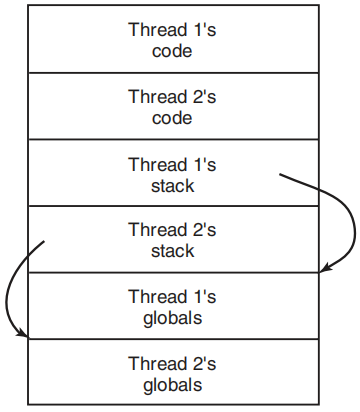
\includegraphics[width=0.85\textwidth]{FIG/2-20.png}
		\caption{进程可以拥有私有的环境变量} \label{fig:privatevariables}
	\end{figure}

	在这种方法下,每一个线程都有私有的errno的副本和全局变量,所以避免了冲突。在效果上,这个方案创造了新的作用域层,这些变量对一个线程中的所有过程都是适用的(但是不涉及其他的过程)。而在原先的作用域层里,变量只对一个过程可见,并在程序中处处可见。
	
	访问私有的全局变量需要一些技巧,不过,多数程序设计语言都有方法表达私有变量和全局变量,但是没有中间的形式。有可能为全局变量分配一块内存,并且把它作为额外的参数传递给线程中的每一个过程。虽然它不是一个优雅的解决方案,但是它是一个可用的方案。
	
	还有一种方案,引入新的库过程,以便创建,设置和读取这些线程范围内的全局变量。首先一个调用是这样的,\texttt{create global("bufptr");}
	
	它在堆上或者在为调用线程保留的特殊区域上为\texttt{bufptr}指针分配存储空间。不管存储被分配到哪里,只有调用线程访问了全局变量。如果另外一个线程创建了一个同名的全局变量,它得到一个与现有存储位置不冲突的不同的存储位置。两个调用都需要访问全局变量,一个用来写它们,一个用来读它们。对于写,类似有set\_global("bufptr", \&buf);它把指针的值存储到之前由\texttt{create \_global}调用创建的存储位置上。为了读取一个全局变量,调用可能像:bufptr = read global("bufptr");
	
	它返回存储在全局变量中的地址,这样可以被访问到数据。试图将单一线程程序转化为多线程程序的另一个问题是,有许多库过程并不是可重入的。也就是说,它们不被设计成在前一个调用尚未完成时对任何给定过程进行第二次调用。例如,在网络上发送一条消息很可能被编程成在库中的一个固定缓冲区中组装消息,然后捕获到内核来发送它。当一个线程已经在缓冲区中组装了消息的情况下将会发生什么。然后时钟中断会强制切换到第二个线程,该线程立即用自己的消息覆盖缓冲区?
	相似地,像UNIX中的内存分配过程\texttt{malloc},维持关于内存使用的关键表格,例如,一个可用内存块的链表。当\texttt{malloc}正忙于更新这些链表,它们可能暂时处在一个不一致的状态,没有指向任何地方的指针。如果在不一致的状态下发生了线程切换,并且从另外一个新的线程产生了一个调用,可能会使用到一个失效指针,而导致程序崩溃。解决好所有的这些问题有效地意味着重写整个库。这样做是一个非常重要的动作,有可能会引入新的错误细节。
	
	另一种解决方案是为每个过程提供一个封套,该封套设置一个位,将库标记为正在使用中。在上一次调用尚未完成时,任何其他线程使用库过程的尝试都将被阻止。尽管这种方法可以工作,但它极大地消除了潜在的并行性。
	
	接下来,我们考虑一下信号。有些信号在逻辑上是线程特定的,而另一些则不是。例如,当一个线程调用\texttt{alarm}的时候,结果信号转到发出调用的线程是有意义的。然而,当线程完全在用户空间实现的时候,内核甚至不知道线程,也很难将信号指向正确的线程。如果一个进程一次只能挂起一个警报,并且多个线程独立地调用警报,则会出现额外的复杂情况。
	
	其他的信号,像键盘中断,并不是线程特定的。谁应该获取它们?是指定的某一个线程,还是所有的线程?还是一个新创建的弹出线程?更多的是,如果一个线程在不通知其他线程的情况下更改了信号处理程序,会发生什么情况?如果一个线程想要捕捉一个特定的信号(比如,用户按CTRL-C键),会发生什么情况呢?还有另一个线程想要这个信号来终止这个进程? 如果一个或多个线程运行标准库过程,而其他线程是用户编写的,则可能会出现这种情况。显然,这些愿望是不能相容的。通常情况下,信号在单线程环境下很难被管理,进入多线程环境中并不一定使得它们更容易被管理。
	
	线程引发的最后一个问题是栈的管理。在许多系统中,当一个进程的堆栈溢出时,内核只是为该进程自动地提供更多的堆栈。当一个进程有多个线程的时候,它必须也有多个堆栈。如果内核对这些堆栈不能完全感知,就不能对它们进行增长直到堆栈出错。事实上,内核有可能还没有意识到内存错误是和某个线程栈的增长有关系的。
	
	这些问题当然不是不可克服的,但他们确实表明,仅仅在现有系统中引入线程而不进行相当实质性的系统重新设计是行不通的。系统调用的语义至少需要重新定义和重写库。所有的这些都必须以这样的一种方式来完成,即对于一个只有一个线程的进程的限制情况,必须保持与现有程序的向后兼容。
	
	关于线程更多的信息,参考Hauser et al. (1993), Marsh et al. (1991), 和Rodrigues et al.
(2010)等人的工作。
	
	\section{进程间通信}
	
	进程总是经常需要和其他的进程进行频繁的通信。例如,在一个shell管道中,第一个进程的输出必须被传递给第二个进程,这就样沿着线一直传下去。这样进程间就有通信的需求,而且最好使用一种良好定义的方法而不是中断。在接下来的章节中,我们将看一下和进程间通信(IPC)相关的主题。
	
	简要地说,这里有三个主题。第一个主题和上面的描述有关,一个进程如何向另一个进程传递信息。第二个主题是确保两个进程在关键性的活动中不会互相冲突,例如,两个进程在飞机的订票系统中同时想为不同的客户抢订一架航班中的最后一张票。第三个主题关注的是当进程间有依赖性的时候其正确的顺序:如果进程A处理数据,进程B打印它们,进程B需要在进程A产生一些数据之前进行一些等待才能开始打印。我们将在开始的章节中探讨这三个问题。
	
	有必要说明的是,这三个问题中的两个问题对于线程来说也是同样重要和适用的。第一个问题-传递信息-这个问题对于线程来说比较容易,因为它们共享同一个地址空间(不同地址空间的线程之间的通信属于进程间通信的范畴)。但是,另外两个问题,需要梳理清楚并保持适当的顺序-同样适用于线程。同样的问题存在可用同样的方法解决。下面开始讨论进程间通信的问题,但是请记住同样的问题和解决方案也适用于线程。
	
	\subsection{竞争条件}
	
	在一些操作系统中,协作的进程可能共享一些彼此都能读写的公用存储区。这些共享存储可能在主内存中(可能在一个内核数据结构中),或者可能是一个共享文件。共享内存的位置并不改变通信的自然属性或者产生的问题。为了理解实际中进程间通信是如何工作的,让我们看一个简单但是常见的例子:一个假脱机打印程序。当一个进程想要打印一个文件,它将文件名放到一个特殊的假脱机目录下。另一个进程(打印机守护线程),则周期性的检查是否有一些文件需要打印,如果有,就打印它们,并把它们的文件名从假脱机目录下删除。
	
	想象一下我们的假脱机目录有很多的槽,从0,1,2...,每一个槽都可以放置一个文件名。同时假设有两个共享变量,\texttt{out}指向要打印的下一个文件,\texttt{in}指向目录中下一个空闲的槽位。这两个变量保存在所有的进程都能够访问的两字的文件中。
	
	在一定特定的时刻,槽位0和槽位3是空的(文件已经被打印了),槽位4和槽位6是满的(有排队待打印的文件名)。差不多在同一时刻,进程A和进程B决定想要排一个文件进行打印,这个情况如图 \ref{fig:sharedmemory} 所示。
	
	\begin{figure}[ht]\small
		\centering
		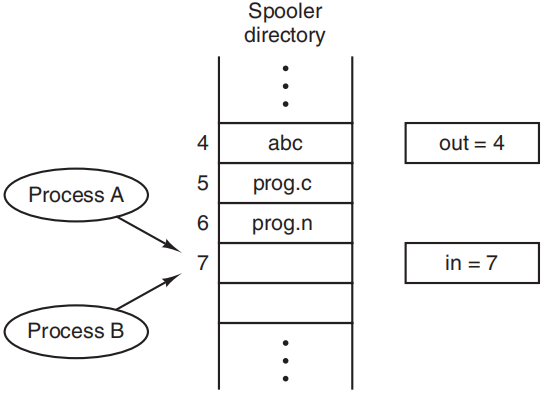
\includegraphics[width=0.85\textwidth]{FIG/2-21.png}
		\caption{两个进程同时想访问共享内存} \label{fig:sharedmemory}
	\end{figure}

	适用于墨菲定律\footnote{如果一件事情有可能会出错,那它就真的会出错。}的管辖区,可能发生接下来的事情。进程A读取\texttt{in}并存储值7,在一个本地变量\texttt{next free slot}。
	就在这时发生了一个时钟中断,CPU认为进程A已经运行了足够长的时间,并决定切换到进程B。进程B同样读取变量\texttt{in},也得到值7,它也把这个值存放到本地变量\texttt{next free slot}中。在这次,两个进程都认为下一个可用的槽位都是7。
	
	进程B接着运行,它把文件名存放在槽7中,并更新\texttt{in}的值为8,它接着做其他的事情。
	
	最后,进程A重新运行,从它离开的位置重新开始运行。它查看\texttt{next free slot}的值,发现其值为7,并把它要打印的文件名放置在槽位7中,擦掉了进程B刚刚放置在那里的名字。接着它计算\texttt{next free slot}+1,得到值为8,并把\texttt{in}设置为8。现在假脱机目录内部是一致的,所以打印守护程序不会察觉到有什么错误,但是进程B将不会再接收到任何的输出了。用户B将会被挂起甚至数年的时间,望眼欲穿地等待输出而它却永远不会来。
	
	类似的这种情况,当两个或更多的进程正在读或者写一些共享的数据,而最终的结果取决于进程运行的精确时序,称为竞争条件(race condition)。调试带有竞争条件的程序可一点都不好玩。大多数的测试运行结果都很好,但是有时候会发生一些意想不到,无法解释的奇怪现象。不幸的是,多核的增长而带来的并行使得竞争条件变得越来越普遍。
	
	\subsection{临界区}
	
	如何来避免竞争条件呢?在这里,以及在许多其他地方涉及共享内存,共享文件和共享所有其他内容的情况下,防止出现问题的关键是找到某种方法来禁止多个进程同时读写共享数据。换言之,我们需要的是互斥(mutual exclusion)。也就是保证当一个进程在使用一个共享变量或者文件的时候,其他的进程将会被排除在做同样的事情的一些方法。出现上面困难情况的原因是进程B在进程A完成之前就使用了共享变量。使用适当的原子操作来实现互斥是任何操作系统设计的一个主要问题,也是后面几节中需要详细讨论的主题。
	
	避免竞争条件的问题还可以通过一种抽象的方式进行描述。一部分时间,进程在做一些内部的计算和其他的一些不会导致竞争条件的事情。但是,有时候内存需要访问共享内存或者文件,或者做一些可能导致竞争条件的其他的关键事情。那部分访问共享内存的程序我们称之为临界区(critical region/critical section)。如果我们可以做一些安排,使得两个进程不会同时处于临界区,我们就可以避免竞争。
	
	尽管这样需要避免竞争的条件,但是这样还不足以保证并发的进程能够正确地协作并有效地利用共享数据。我们需要坚持四个条件来形成一个好的解决方法:
	
	1. 没有两个进程可以同时在它们的临界区。 
	2. 不应对CPU速度和个数做任何的假设。
	3. 正在运行在其临界区之外的进程不能阻塞其他任何进程。
	4. 不得使进程无限期地等待进入其临界区。
	
	从一个抽象的角度看,我们想要的行为方式在图 \ref{fig:mutualexclusion} 中展示了出来。
	
	\begin{figure}[ht]\small
		\centering
		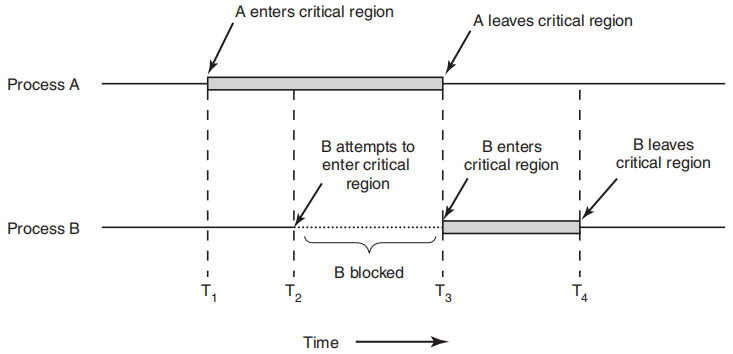
\includegraphics[width=0.90\textwidth]{FIG/2-22.png}
		\caption{使用临界区的互斥} \label{fig:mutualexclusion}
	\end{figure}

	在这张图中,进程A在时间T1进入临界区,稍候,在时间T2进程B尝试进入临界区但是失败了,因为已经有一个进程在临界区,我们在某一个时刻只允许有一个进程在临界区。结果,进程B被暂时挂起,直到时刻T3,进程A离开了临界区,并立即允许进程B进入临界区。最终,进程B在T4时刻也离开了临界区,我们也回到了最初没有进程在其临界区的状态。
	
	\subsection{带忙等待的互斥}
	
	在本节中,我们将研究互斥的各种方案,这样,当一个临界区正忙于更新在其临界区中的共享内存,没有其他的进程将进入临界区并导致麻烦。
	
	\textbf{1. 屏蔽中断}
	
	在一个单处理器系统中,最简单的方法是对每一个进程在它进入临界区后就立即禁用中断,并在它离开临界区的时候再启用中断。屏蔽中断后,时钟中断也被屏蔽。毕竟,CPU只在时钟中断或其他中断的情况下才会从一个进程切换到另一个进程,在中断关闭的情况下CPU不会从一个进程切换到另外一个进程。
	
	所以,一旦CPU屏蔽了中断,它可以大胆地检查和更新共享内存,而不用担心别的进程会干扰。这种方法通常是没有吸引力的,因为给用户进程关闭中断是不明智的。如果它们中的一个进程关闭了中断而再也没有打开它们怎么办?整个系统可能会因此终止。此外,如果系统是一个多处理器(有两个或多个CPU)的系统,禁用中断只会影响执行禁用指令的CPU,其他的CPU可以继续运行并访问共享内存区域。
	
	另一方面,内核本身在更新变量或特别是列表时,常常可以方便地为一些指令禁用中断。例如,如果在就绪进程列表处在不一致的状态下发生了中断,则就有可能发生竞争条件(race condition)。结论是:禁用中断通常是操作系统本身一项有用的技术,但是并不适合作为用户进程的一种合适的通用互斥机制。即使是在内核中,通过禁用中断来实现互斥的可能性也越来越小,因为多核芯片的数量在低端的PC机器上也越来越多了。两个核心的已经很普遍了,四个核心的在很多机器上也有了,8个,16个甚至32个核心的也不远了。在一个多处理器的系统中,禁用一个CPU的中断并不能防止其他的CPU干预第一个CPU所做的操作,结果是人们需要更复杂的方案。
	
	\textbf{2. 锁变量}
	
	作为第二个尝试,让我们来看一个软件的解决方法。考虑使用一个共享变量,初始值为0。当一个进程尝试进入它的临界区的时候,它首先测试这个锁。如果这个锁为0,则进程将它设置为1并进入临界区。如果锁已经是1了,则进程仅仅只是等待它变为0。所以,值为0意味着没有进程在其临界区,值为1意味着有一些进程在其临界区。
	
	但是,这个想法有一个类似于假脱机目录一样的致命错误。假设一个进程读取了锁并发现它为0,在它被设为1之前,另外一个进程调度,运行并把它设置为1了。当第一个进程再次运行的时候,它同样把它设置为1,这样两个进程都会同时在临界区上。
	
	现在您可能认为我们可以通过先读取锁值,然后在存储到它之前再次检查它来解决这个问题,但这确实没有帮助。现在,如果第二个进程在第一个进程完成第二次检查之后修改了锁,则会发生竞争条件。
	
	\textbf{3. 严格轮换法}
	
	第三种互斥的方法如图 \ref{fig:strictalternation} 所示。几乎和本书的所有的其他程序段一样,这个程序段也是用C语言编写的。我们在这里选用C语言是因为实际的操作系统都是用C语言(或者是C++)编写的,但是很少有用Java,Python或者是Haskell编写的。C语言强大,有效,可预见而且有特性。对于Java,则不可预见,它有能在关键时刻使用完了内存,从而需要一个不合适的时间启动垃圾回收器。这在C语言中是不会发生的,因为C语言中没有垃圾回收。 Prechelt(2000)给出了一个关于C,C++,Java以及其他四种语言的定性比较。
	
	\begin{figure}[ht]\small
		\centering
		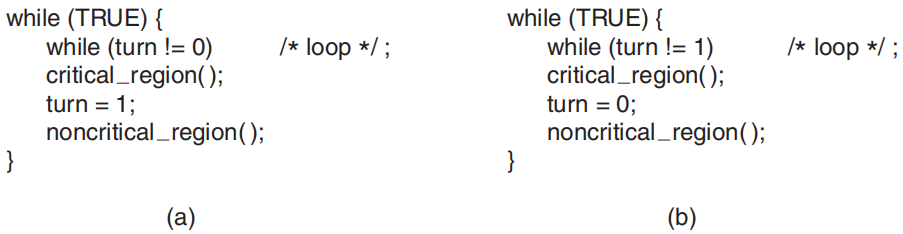
\includegraphics[width=0.90\textwidth]{FIG/2-23.png}
		\caption{一种临界区问题的解决方案。请注意,在两种情况下分号都中止了while循环。a) 进程0,b) 进程1。} \label{fig:strictalternation}
	\end{figure}
	
	在图 \ref{fig:strictalternation} 中,整数变量turn(最初为0)跟踪轮到谁进入临界区并检查或更新共享内存。一开始,进程A检测\texttt{turn},发现它为0,并进入它的临界区。进程1也同样发现它是0,于是在一个等待循环中不停地测试\texttt{turn},看它何时会变为1。不断地测试一个值知道某一个值的出现,称之为忙等待(busy waiting)。
	
	它通常是应该被避免的,因为它浪费CPU的时间。只有在有一个合理的预期说明这个等待是短暂的才会使用忙等待。一个使用忙等待的锁称之为自旋锁(spin lock)。
	
	当进程0离开了临界区,它将\texttt{turn}设置为1,并允许进程1进入其临界区。假设进程1很快地结束了其临界区,这样两个进程都不再它们的临界区中了,\texttt{turn}被设置为0。现在进程0很快地执行整个循环,退出临界区并设置\texttt{turn}为1。在这个时间点,\texttt{turn}的值为1,并且两个进程都执行在它们的非临界区上。
	
	突然,进程0结束了非临界区的操作并且返回到循环的开始。但是,它此时不被允许进入临界区,因为\texttt{turn}此时为1,进程1正在它的非临界区运行。进程0只有继续循环,直到进程1将\texttt{turn}设置为0。换言之,当一个进程比另一个进程慢地多的时候,轮流并不是一个好主意。这种情况违反了上面列出的条件3:进程0被一个不在其临界区内的进程阻塞。回到上面讨论的假脱机目录,如果我们将临界区和读写假脱机目录关联起来,进程0将不被允许打印另外一个文件因为进程1正在做其他的事情。
	
	事实上,这个方法需要两个进程严格交替地进入它们的临界区,如假脱机文件等。任何一个进程都不能在一轮中打印两个文件。尽管这个算法避免了竞争,但是它并不是一个严格意义上的解决方案因为其违反了规则3。
	
	\textbf{4. Peterson解法}
	
	通过综合锁变量和警告变量的想法,荷兰数学家T. Dekker第一个提出了不需要严格轮换的的互斥问题的软件解法。关于T. Dekker的算法,请参照Dijkstra(1965)。
	
	1981年,Peterson发现了一种简单得多的互斥算法,这使得Dekker的算法变得过时了。Peterson的算法在图 \ref{fig:peterson} 中展示了出来。
	
	\begin{figure}[ht]\small
		\centering
		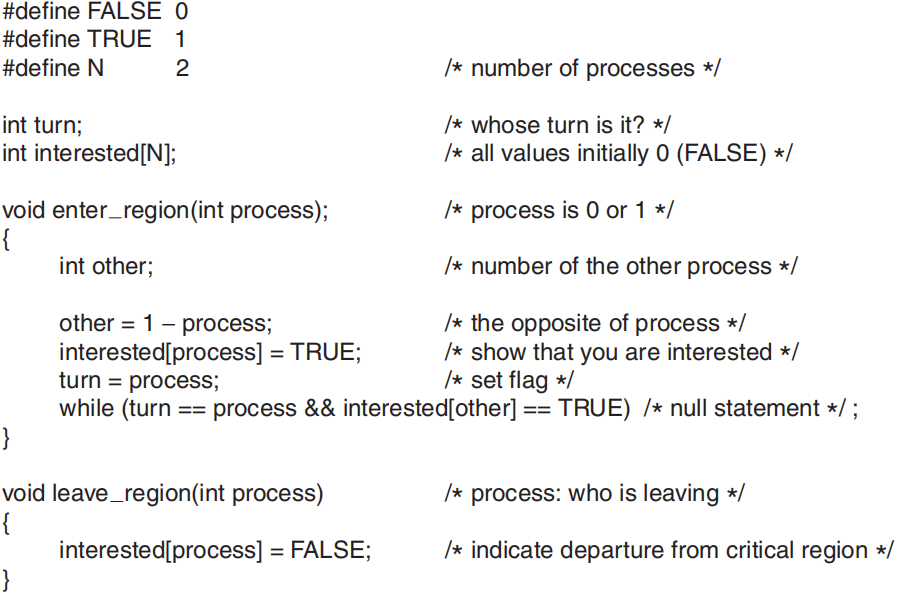
\includegraphics[width=0.90\textwidth]{FIG/2-24.png}
		\caption{Peterson算法} \label{fig:peterson}
	\end{figure}

	这个算法由两个由C语言写的过程组成。这意味着应该为定义和使用的所有函数提供函数原型。但是,为了节省空间,我们不会在这里或以后展示原型。
	
	在使用共享变量之前(在进入其临界区之前),每一个进程使用他们的进程号0或1作参数调用\texttt{enter\_region}。这个调用将会导致它的等待,如果需要的话,直到可以安全地进入临界区。当它完成了对共享变量的操作,进程调用\texttt{leave\_region}以表示它已经离开了临界区并可以允许其他进程进入了,如果有其他进程想进入的话。
	
	让我们看看这个解决方案是如何工作的,一开始没有一个进程是在其临界区之内的。现在进程0调用了\texttt{enter\_region},它通过设置其数组元素和将\texttt{turn}设置为0来表明它想进入临界区。因为进程1并不想进入临界区,所以\texttt{enter\_region}立即返回。如果进程1现在想执行一个\texttt{enter\_region}调用,它将被挂起直到interested[0]变为FALSE,这个情形只有在进程0调用\texttt{leave\_region}退出临界区的时候才会发生。
	
	现在考虑一下进程几乎同时调用\texttt{enter\_region}进入临界区的情形。它们都将进程号存储在变量\texttt{turn}中。但是只有后被保存的进程号才有效,前一个会被重写并丢失。假设进程1是后存入的,则turn为1。当两个进程都来到\texttt{while}语句,进程0执行\texttt{while}0次并进入临界区。进程1循环不进入临界区直到进程0退出临界区。
	
	\textbf{5. TSL指令}
	
	现在我们来看一下需要硬件支持的一种方案。一些计算机,特别是那些设计为多处理器的计算机,都有下面一条指令:TSL RX,LOCK(Test and Set Lock),该指令是这样工作的。它将内存字\texttt{lock}的值读出并放到寄存器\texttt{RX}中,接着在内存地址\texttt{lock}处存储一个非零的值。读字和存储字的操作是不可分割的,没有其他的处理器可以访问该内存字直到这条指令被执行完成。执行TSL指令的CPU锁定内存总线,以禁止其他CPU访问内存,直到它完成。
	
	值得注意的是,锁定内存总线和屏蔽中断有很大的不同。屏蔽中断将对一个内存字先执行一个读操作,再执行一个写操作,但是这并能防止第二个CPU对总线上的内存字执行读和写的操作。事实上,在处理器1上屏蔽中断对处理器2没有任何的影响。放置处理器2访问内存的唯一方法是知道处理器1结束访问总线。需要一个特殊的硬件设施(基本上,如果一个总线声称总线被锁定了,则这个总线除了对锁定它的处理器之外,对其他处理器是不可见的)。
	
	为了使用TSL指令,我们将使用一个共享变量,\texttt{lock},当lock为0时,任何进程都可以使用TSL指令将其设置为1,然后读或写共享内存。完成后,进程使用普通的move指令将lock设置为0。
	
	为什么这条指令可以防止两个进程可以同时进入它们的临界区?方法在图 \ref{fig:tsl} 中给出了。这里展示了一个虚拟(但典型的)汇编语言中的四指令子程序。第一条指令将旧的lock值复制到寄存器,然后将lock设置为1,接着将旧的值和0进行比较。如果它不是零,那么锁已经设置好了,所以程序只会回到开始处并再次测试它。
	
	\begin{figure}[ht]\small
		\centering
		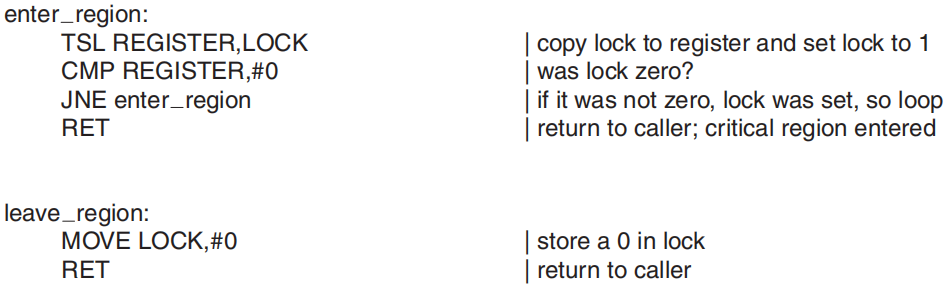
\includegraphics[width=0.90\textwidth]{FIG/2-25.png}
		\caption{使用TSL指令进入和离开临界区} \label{fig:tsl}
	\end{figure}
	
	它迟早会变为0,当前处于其临界区的进程已使用其临界区完成,并且子程序返回时设置了锁。很明显,锁是非常简单的。程序只是在lock中存储了一个0,不需要特殊的同步指令。
	
	应对临界区问题的解决方案现在也非常简单了。在进入它的临界区之前,一个进程调用了\texttt{call\_region},在锁释放之前进行忙等待,接着它需要锁并返回。在退出临界区之前,进程调用\texttt{leave\_region}并在lock中存储0。和其他的基于临界区的解决方案一样,为了使得该方法工作,进程必须调用\texttt{enter\_region}和\texttt{leave\_region}正确的次数。
	
	如果有一个进程欺骗,则互斥将会失败。换句话说,临界区问题的正确解决只有在进程之间相互合作的时候才可以完成。
	
	TSL指令的一个替换指令是XCHG,它原子性地交换两个位置的内容,例如,一个寄存器和一个内存字。代码如图 \ref{fig:xchg} 所示。
	
	\begin{figure}[ht]\small
		\centering
		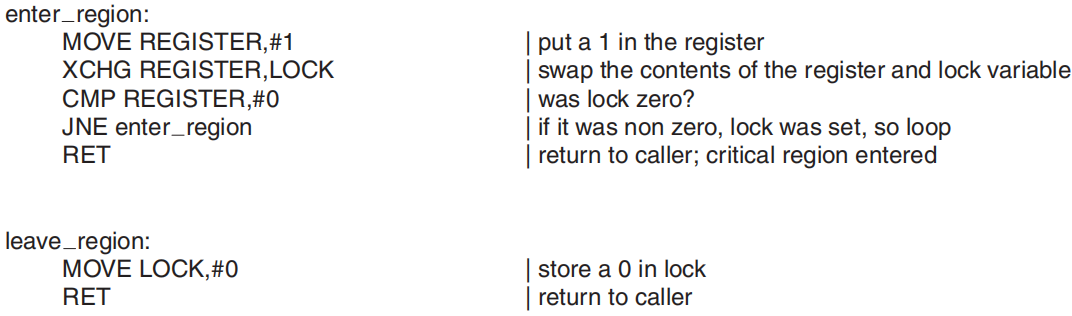
\includegraphics[width=0.90\textwidth]{FIG/2-26.png}
		\caption{使用XCHG指令进入和离开临界区} \label{fig:xchg}
	\end{figure}

	可见,本质上与TSL的解决方案相同,所有Intel x86 CPU都使用XCHG指令进行低级同步。

	\subsection{睡眠与觉醒}
	
	不管是Peterson算法还是使用\texttt{TSL}和\texttt{XCHG}指令的方法都是正确的,但是它们都有需要忙等待的方法。本质上,这些解决方法所做的是:当一个进程进入其临界区,它检查是否允许输入。如果不是,则进程进入一个密集的循环等待,直到它是。
	这种方法不仅浪费CPU的时间,而且还有可能有意想不到的影响。考虑一个有两个进程的计算机,一个进程的优先级高,另一个进程的优先级低。调度的规则是,只要H处在就绪状态就立即运行它。在一个特定的时刻,L在临界区中,H变为就绪准备运行(一个I/O操作完成)。H现在开始忙等待,但是由于H在运行的时候L不会被调度,L永远得不到离开其临界区的机会,所以H就进入了无限循环。这种情况有时候被称为优先级反转问题。
	
	现在让我们看看一些进程间通信原语,它们在不允许进入关键区域时阻塞而不是浪费CPU时间。有一个最简单的组合是\texttt{sleep}和\texttt{wakeup}。\texttt{sleep}是一个导致调用者阻塞的系统调用,会挂起直到另外一个进程将其唤醒。\texttt{wakeup}有一个参数,需要唤醒的进程。另外,\texttt{sleep}和\texttt{wakeup}都有一个参数,一个用于匹配\texttt{sleep}和\texttt{wakeup}的内存地址。
	
	\textbf{生产者-消费者问题}
	
	作为这些原语如何被使用的例子,让我们来考虑一下生产者和消费者问题(也被称为有界缓冲区问题)。两个进程共享一个共同的,固定大小的缓冲区。其中生产者进程,向缓冲区中放入信息,另一个消费者进程,则从缓冲区中取出信息(当然还可以把这个问题一般化为m个生产者和n个消费者,但是我们只考虑一个生产者和一个消费者的情形,因为这样会简化问题)。
	
	当生产者想在缓冲区中放入一个新的项目,但它已经满了,就会出现问题。解决的方法是让生产者去休眠,并且当消费者移除一个或多个项目的时候唤醒它。类似的,如果消费者想从缓冲区中移除一个项目,并且看到缓冲区是空的,它则转入休眠状态,直到生产者将一些项目放入缓冲区并唤醒它。
	
	这个方法显得足够简单,但是它会导致类似之前的假脱机目录类似的竞争条件问题。为了跟踪缓存区中的项目数,我们需要一个变量,\texttt{count}。如果在缓冲区中可以放置的最大项目数目是N,生产者的代码首先检测\texttt{count}的值是否为n,如果是,生产者进程将休眠,如果不是,生产者将增加一个项目并将\texttt{count}的量加1。
	
	消费者的代码是类似的:首先检测一下\texttt{count}的值是否为0,如果是,则休眠,如果不是,则移走一个项目并把\texttt{count}的值减1。每个进程也会测试是否应该唤醒另一个进程,如果应该,则将其唤醒。消费者和生产者进程的代码如图 \ref{fig:producerconsumer} 所示。
	
	\begin{figure}[ht]\small
		\centering
		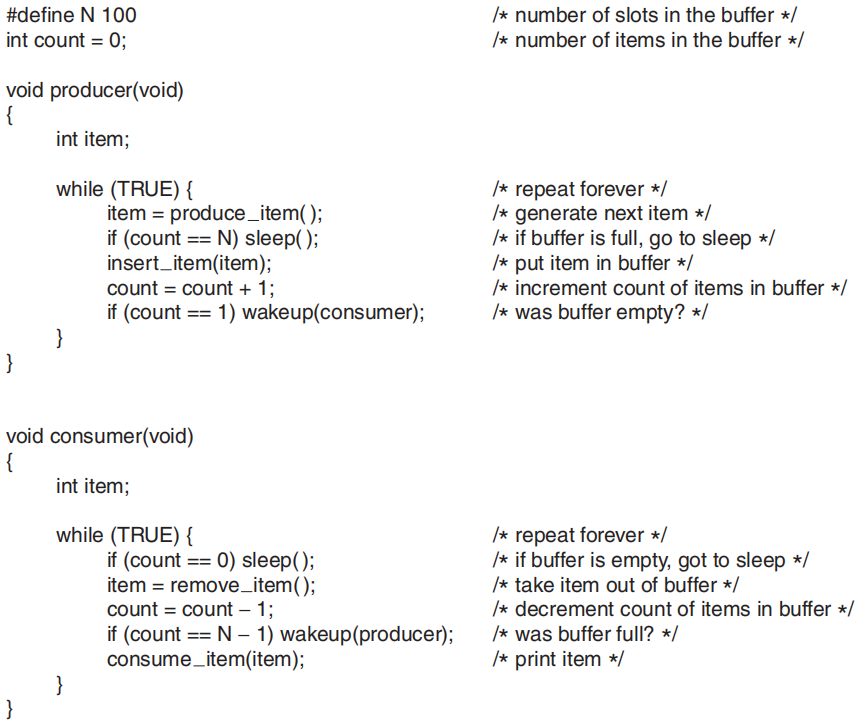
\includegraphics[width=0.90\textwidth]{FIG/2-27.png}
		\caption{生产者消费者问题带有一个致命的竞争条件问题}\label{fig:producerconsumer}
	\end{figure}
	
	为了用C语言来写像\texttt{sleep}和\texttt{wakeup}的系统调用,我们将把它们显示为对库例程的调用。它们不是标准C语言的库,但是可以推测可以在任何有这些系统调用的系统上使用。\texttt{insert item}和\texttt{remove item}过程,未显示的,处理入库和出库的记账。
	
	现在让我们回到竞争条件。它是可以出现的,因为对\texttt{count}的访问是不受限制的。结果,可以出现接下来的情况。缓冲区是空的,消费者进程刚刚读取了\texttt{count}的值并看它是否为0。就在这个时刻,调度器决定暂时停止运行消费者进程并开始运行生产者进程。生产者进程向缓冲区中插入了一个项目,并增加变量\texttt{count}的值,并发现现在它的值是1了。因为\texttt{count}的值为0,因此消费者进程必须处于休眠状态,生产者调用\texttt{wakeup}并唤醒消费者。
	
	但是,消费者此时在逻辑上并没有睡眠,因此\texttt{wakeup}信号消失。当消费者下次运行的时候,它将检测它之前读取的\texttt{count}的值,发现其为0,则继续睡眠。迟早生产者会填满缓冲区也走向睡眠。这样生产者和消费者都永久地休眠了。
	
	问题的症结在于发给一个未睡眠进程的唤醒信号丢失了。如果它没有丢失,则一切都将正常。一个快速的解放方法是修改规则,在上面的场景中添加一个唤醒等待位。当一个唤醒信号被发送给一个清醒的进程的时候,这个位将被设置。稍后,当这个进程想要休眠的时候,如果唤醒等待位是ON,则将其关闭,但是这个进程仍然保持清醒。唤醒等待位是一个存储唤醒信号的银行。消费者在循环的每次迭代中清除唤醒等待位。
	
	尽管在这个简单的例子中唤醒等待位方法解决了问题,但是当有两个或者两个以上的进程共用一个唤醒等待位的时候,将出现唤醒等待位不足的情况。我们可以再做一个补丁,再增加一个唤醒等待位,甚至8个或者32个,但是从原则上讲,并没有根本地解决问题。
	
	\subsection{信号量}
	
	这是在1965年,当E. W. Dijkstra(1965)建议使用一个整型变量来计数唤醒线程的数量并保存用于后来使用。在他的方法中,一个新的变量类型,他称为semaphore,被介绍了。信号量的值可以为0,标志着没有唤醒的进程,如果一个或多个唤醒挂起,则为正值。
	
	Dijkstra提出了对信号量的两个操作,通常被称为\texttt{down}操作和\texttt{up}操作(分别是一般化后的sleep和wakeup操作)。对于一个信号量的\texttt{down}操作检查信号量的值是否大于0。如果是,它减少信号量的值(唤醒)并继续。如果该值为0,则进程将进入休眠状态,暂时不完成关闭。检查信号量的值,改变它,并有可能休眠,都是在一个单个的,不可分割的原子操作(atomic action)中完成的。它就保证了当一个进程对信号量进行操作的时候,则没有其他的进程可以访问信号量直到该操作被完成为止。这种原子性对于解决同步问题和避免竞争条件是完全必要的。原子操作,其中一组相关的操作要么全部不中断地执行,要么根本不执行,在计算机科学的许多其他领域也是极其重要的。
	
	\texttt{up}操作增加所寻址信号量的值。如果有一个或者更多的进程在那个信号量上休眠,则不能结束一个更早的\texttt{down}操作,其中有一个是被系统选择(随机的),并允许结束它的\texttt{down}。因而,在有进程休眠的信号量上执行\texttt{up}操作后,信号量将变为0,但是这样会减少一个睡眠的进程。增加信号量和唤醒一个进程的操作同样是不可分割的。没有进程阻塞\texttt{up}操作,就像早期的模型中没有进程阻塞\texttt{wakeup}一样。
	
	作为一个补充,在Dijkstra早期的论文中,它使用了P和V的名称分别代替了\texttt{down}和\texttt{up}。因为这些对不说荷兰语的人们没有感知,并且对只做Proberen操作(尝试)和Verhogen操作(升高)-我们将使用术语\texttt{down}和\texttt{up}代替。它们在程序设计语言Algol86中首次被引入。
	
	\textbf{使用信号量解决生产者-消费者问题}
	
	信号量解决\texttt{wakeup}丢失问题,如图 \ref{fig:semaphores} 所示。
	
	\begin{figure}[ht]\small
		\centering
		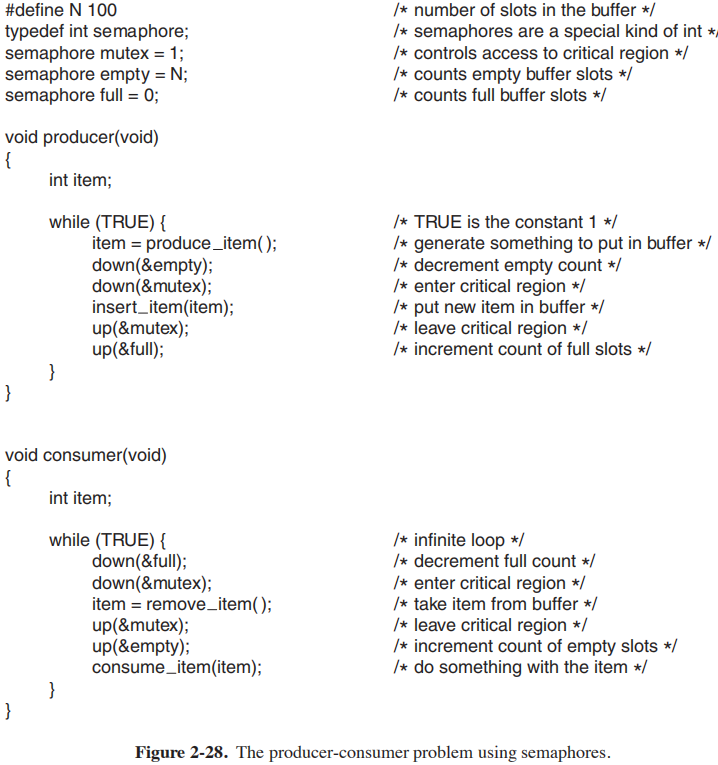
\includegraphics[width=0.90\textwidth]{FIG/2-28.png}
		\caption{使用信号量的生产者和消费者问题}\label{fig:semaphores}
	\end{figure}
	
	要使得它们正常地工作,必须将它们以不可分割的方式实现。通常的方式是将\texttt{up}和\texttt{down}操作实现为系统调用,而且操作系统在执行以下操作的时候暂时禁用所有的中断:测试信号量,更新信号量,将线程睡眠等。所有的这些操作只需要几条指令,并且禁用中断也不会造成什么伤害。如果使用了多个CPU,每一个信号量应该被一个锁变量保护,通过TSL和XCHG操作确保在一个时刻只有一个CPU对信号量进行操作。
	
	请确保你懂得使用TSL或者XCHG指令来防止多个CPU同时访问信号量,和生产者和消费者的忙等待另一方填充或者清空缓冲区是大不相同的。信号量操作可能只会占用几毫秒的时间,而生产者和消费者可能要占用更长的时间。
	
	这个方案使用了三个信号量: 一个调用\texttt{full}来计算满的槽位的个数,一个调用\texttt{empty}来计算空的槽位的个数,另一个调用\texttt{mutex}来保证生产者和消费者不同时访问buffer。Full的初始值是0,empty的初始值等于缓冲区中槽的个数,mutex的初始值为1。初始化值为1,由2个或更多的进程使用,并且保证在同一时刻只有一个进程进入其临界区的信号量,称为二进制信号量。
	
	如果每一个线程在进入临界区之前执行一个\texttt{down}操作,在离开临界区之后执行一个\texttt{up}操作,则就可以保证互斥。
	
	现在我们有了一个好的中断原语,让我们回到图 \ref{fig:interupt} 所示的中断序列中来。如果一个系统使用信号量,则隐藏中断的一个自然的方法是有一个信号量,初始值设置为0,和每一个I/O设备关联。在开启了一个I/O设备之后,管理进程在与之相关联的信号量上做一个\texttt{down}操作,接着就立即阻塞。当中断进来的时候,中断处理器在相应的信号量上做\texttt{up}操作,使得相关的进程重新进入就绪态。在这个模型中,图 \ref{fig:interupt} 中的步骤5包含了在设备的信号量上做一个\texttt{up}操作,这样在步骤6中调度器就可以运行设备管理器了。当然,如果几个进程现在都就绪了,调度器接下来可能会选择一个更加重要的进程。我们将在本章接下来的看几个用于调度的算法。
	
	在图 \ref{fig:semaphores} 的例子中,我们实际上使用两种不同的方式来使用信号量。弄清楚两者之间的区别是非常重要的。\texttt{mutex}信号量用于互斥,它被设计为一个只有一个进程读写缓冲区和相关的变量。这个互斥被要求用来防止混乱。我们在接下来的章节中将研究互斥。
	
	信号量的另一个用途是同步,需要完整和空的信号量来保证特定的事件序列发生或者不发生。在这种情况下,它保证当缓冲区满的时候生产者进程停止运行,当缓冲区空的时候消费者进程停止运行。这个使用方法不同于互斥。
	
	\subsection{互斥量}
	
	当不需要信号量的计数能力的时候,有时候会使用信号量的简化版本,称为互斥量。互斥量只管理一些共享资源和代码段的互斥。
	
	互斥量是一个可以有两种状态的共享变量:锁定或者非锁定。因此,只需要1位就可以表示,但是实际上通常使用整数,用0表示非锁定,其他值表示锁定。
	
	两个过程用于互斥量。当一个线程(或者进程)需要访问临界区的时候,它调用\texttt{mutex\_lock}。如果互斥量当前是非锁定的(意味着临界区是可用的),则调用成功,调用线程可以自由地出入临界区。
	
	另一方面,如果互斥量已经被锁定了(意味着临界区是可用的),则调用线程被阻塞直到临界区中的线程结束并调用\texttt{mutex\_unlock}。如果多个线程在互斥锁上被阻塞,则随机选择其中一个线程并允许获取锁。 
	
	因为互斥量是如此地简单,它们可以在用户空间轻易地使用TSL或者XCHG指令来实现。\texttt{mutex\_lock}和\texttt{mutex\_unlock}和带有一个用户级线程包的代码如图 \ref{fig:mutex} 所示。带有XCHG的实现方案是完全相同的。
	
	\begin{figure}[ht]\small
		\centering
		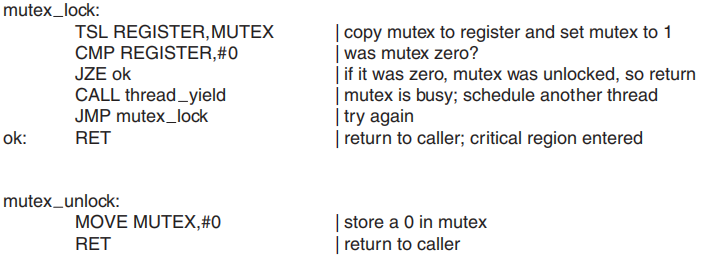
\includegraphics[width=0.90\textwidth]{FIG/2-29.png}
		\caption{mutex\_lock和mutex\_unlock的实现} \label{fig:mutex}
	\end{figure}
	
	\texttt{mutex\_lock}的代码和图 \ref{fig:tsl} 中\texttt{enter\_region}的代码非常类似。当\texttt{enter\_region}进入缓冲区失败,它将保持重复地测试锁(忙等待)。
	最终,时钟用完了,其他进程将被安排运行。持有锁的进程迟早会运行并释放它。对于(用户)线程,情况有所不同,因为没有时钟可以阻止线程运行这么长的时间。
	
	这就是\texttt{enter\_region}和\texttt{mutex\_lock}的区别。当稍后请求一个锁失败,它调用\texttt{thread\_yield}来放弃CPU给另外一个线程。因此,没有忙等待。当线程下次运行时,它将再次测试锁。
	
	因为\texttt{thread\_yield}仅仅是在用户空间中进程调度器的一个调用,它的速度非常快。这样,\texttt{mutex\_lock}和\texttt{mutex\_unlock}都不需要任何的内核调用。使用它们,用户级线程完全可以实现在用户空间中的同步,这些过程仅仅需要少量的指令。
	
	我们上面描述的mutex系统仅仅是一套调用。对于所有的软件,总是需要更多的特性,同步原语也不例外。有时线程包提供一个调用互斥锁trylock,它要么获取锁,要么返回失败代码,但不阻塞。这个调用使线程能够灵活地决定下一步要做什么,如果除了等待之外还有其他选择。
	
	到目前为止,我们隐藏了一个问题,不过现在还是有必要把这个问题提出来。对于用户空间线程包,多个线程访问同一个互斥体没有问题,因为所有线程都在一个公共地址空间中运行。对于早期的解决方案,如Peterson算法和工作量,有一个不言而喻的假设,即多个进程至少可以访问一些共享内存,也许只有一个字,但有些东西。如果进程有不相交的地址空间,就像我们一直说的那样,它们如何共享Peterson算法中的turn变量、信号量或公共缓冲区? 
	
	这里有两个答案。第一,是一些共享的数据结构,像信号量,可以存储在内核中,只能通过系统调用访问,这个方法消除这个问题。其次,大多数现代操作系统(包括UNIX和Windows)都提供了一种方法,让进程与其他进程共享部分地址空间。在这种方法,缓冲区和其他数据结构可以共享。在最坏的情况下,一个文件是不能被共享的。
	
	如果两个或者更多的线程共享了它们的地址空间,进程和线程之间的区别将会变得比较模糊但是仍旧会存在。共享同一地址空间的两个进程仍具有不同的打开文件、警报计时器和其他每个进程属性,而单个进程中的线程共享这些属性。共享一个公共地址空间的多个进程从来没有像用户级线程那样高效,因为内核与它们的管理密切相关。
	
	\textbf{快速用户区互斥量}
	
	随着并行度的提高,高效的同步和锁定对性能是非常重要的。如果等待比较短自旋锁是快速的,但是如果不是,则就会浪费CPU的时间。因此,如果存在大量争用,那么阻塞进程并让内核在锁空闲时解除阻塞会更有效。不幸的是,这里有一个相反的问题:在重度争用的情况下工作地非常好,但是持续地切换至内核是非常昂贵的,如果只有很少的争用的话。令事情更加糟糕的是,预测锁争用的量可能就不容易了。
	
	一个试图综合这两个世界最好的方法是"futex",或者称为"快速用户空间互斥"。futex是Linux实现了基本锁机制(更像是互斥)的一个特性,但是避免陷入内核除非它必须陷入。因为切换回内核是非常昂贵的,所以这样做可以很好地改善性能。一个用户空间互斥包含两部分内容:一个内核服务和一个用户库。内核服务提供一个"等待队列",允许多个线程在一个锁上进行等待。它们不会运行,除非内核显式地解锁它们。将进程放入等待队列需要(昂贵的)系统调用,应该避免。在没有争用的情况下,所以,用户空间互斥完全工作在用户空间。
	
	特别地,这些进程共享一个通用的锁变量—一个用作锁的32位对齐的整数的别名。假设,锁的初始值为1,这意味着锁是自由的。一个线程通过执行一个原子性的"减量和测试"(Linux中的原子函数由封装在C函数中的内联程序集组成,并在头文件中定义)。 接下来,线程检查结果以查看锁是否空闲。如果它不在锁定状态,则一切正常,线程已经成功地捕获了锁。然而,如果该锁被另外一个线程所持有,则我们的线程则必须等待。在这种情况下,用户空间互斥库并没有自旋,但是使用系统调用将线程放到内核中的等待队列中。更有希望的是,现在切换到内核的代价是合理的,因为线程无论如何都被阻塞了。当线程完成了锁操作以后,它使用一个"增量并测试"释放了锁,并检查结果以查看内核等待队列上是否仍有任何进程被阻塞。如果是这样的话,它会让内核知道它可能会解除对这些进程中的一个或多个的阻塞。如果没有争用,则根本不涉及内核。
	
	\textbf{Pthreads中的互斥量}
	
	Pthreads提供了一组可以用来同步线程的函数。基本机制使用互斥变量(可以锁定或解锁)来保护每个关键区域。一个想进入临界区的进程首先尝试锁定与其相关联的互斥量。如果互斥量是非锁定的,进程可以理解进入并且锁被自动设置,从而防止其他的进程进入。
	如果互斥量已经锁定了,则调用线程阻塞直到它失去锁定。如果多个线程在等待同一个互斥量,当它被解锁的时候,只有一个线程允许继续运行并对其重启锁定,这些锁并不是必须的。由程序员来确保线程正确地使用它们。
	
	\begin{figure}[ht]\small
		\centering
		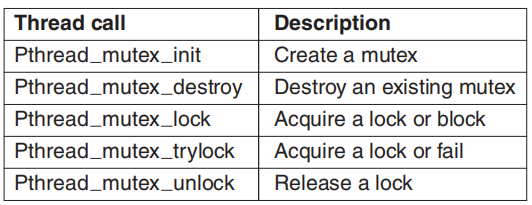
\includegraphics[width=0.90\textwidth]{FIG/2-30.png}
		\caption{和互斥量相关的Pthreads进程} \label{fig:pthreadsmutex}
	\end{figure}
	
	关于互斥量的主要调用如图 \ref{fig:pthreadsmutex} 中所示。和预期的一样,互斥量可以被创建和销毁。进行创建和销毁操作的线程分别是\texttt{pthread\_mutex\_init}和\texttt{pthread\_mutex\_destory}。它们同样可以被\texttt{pthread\_mutex\_lock}锁定,该调用尝试获得锁并在已经获得锁的情况下进行阻塞。
	Pthreads提供了许多可以用来同步线程的函数。基本机制使用互斥变量(可以锁定或解锁)来保护每个关键区域。还有一个选项,用于尝试锁定互斥锁,但如果互斥锁已被阻止,则返回错误代码而不是阻塞。这个调用是\texttt{pthread\_mutex\_trylock}。此调用允许线程在需要时有效地执行忙等待。
	最后,\texttt{pthread\_mutex\_unlock}解锁一个互斥锁,如果一个或多个线程正在等待它,则只释放一个线程。互斥锁也可以有属性,但是这些属性只用于特殊目的。
	
	除了互斥量,Pthreads还提供了第二种同步机制:条件变量。互斥锁有助于允许或阻止对临界区的访问。条件变量运行线程由于某些条件不满足而阻塞。几乎两个方法都是同时使用的。让我们更加仔细地看一下线程,互斥量和条件变量的相互关联。
	
	最为一个简单的例子,重新考虑一下生产者和消费者的情形:一个线程放置物品到缓冲区,另一个线程将它们取出。如果生产商认为缓冲区没有可用的空闲插槽,则它将阻塞直到有一个空闲插槽为止。互斥锁可以在不受其他线程干扰的情况下以原子方式进行检查,如果发现缓冲区已经满了,则生产者需要阻塞并且在稍后唤醒,这就是条件变量所允许的。
	
	和条件变量最相关的调用如图 \ref{fig:conditionvariables} 所示。
	
	\begin{figure}[ht]\small
		\centering
		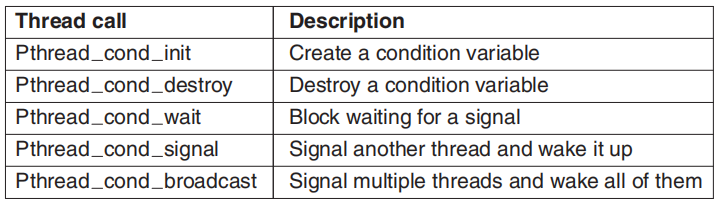
\includegraphics[width=0.90\textwidth]{FIG/2-31.png}
		\caption{一些和条件变量相关的Pthreads调用} \label{fig:conditionvariables}
	\end{figure}
	
	可能和你期待的一样,这里有创建和销毁条件变量的调用。它们可以有属性,而且有各种不同的调用来管理它们(没有列出)。对条件变量的主要操作是\texttt{pthread\_cond\_wait}和\texttt{pthread\_cond\_singal}。
	前者阻塞调用线程,直到其他线程向它发出信号(使用后一个调用)。当然,阻塞和等待的原因不是等待和发信号协议的一部分。阻塞线程通常等待发信号线程做一些工作,释放资源或者执行一些其他的活动。只有完成后被阻塞的线程才可以继续进行,条件变量允许这个等待和阻塞原子性地完成。当多个线程被阻塞并等待同一个信号时,可以使用\texttt{pthread\_cond\_broadcast}调用。
	条件变量和互斥总是在一起被使用的。模式是一个线程锁定一个互斥量,等待一个条件变量但是用不能得到它想要的。最后另外一个线程将发出信号,它可以继续。
	\texttt{pthread\_cond\_wait}可以原子性地解锁它所持有的互斥量。因为这个原因,mutex是其中的一个参数。同样值得注意的是条件变量(不同于信号量)没有内存。如果一个信号被发送给一个没有线程等待的条件变量,信号将会丢失。编程者必须小心地不弄丢信号。
	
	作为互斥量和条件变量如果被使用的例子,图 \ref{fig:thread-producer-consumer} 给出了一个简单的带有一个单缓冲区的生产者和消费者问题。当生产者已经填充满缓冲区,它必须等待消费者将其清空后才能够填充新的条目。类似地,当消费者移除一个条目的时候,它必须等待生产者产生另外一个条目。尽管非常简单,这个例子阐述了基本的机制。使线程进入睡眠状态的语句应始终检查条件,以确保在继续运行之前满足该条件,因为该线程可能由于UNIX信号或其他原因而被唤醒。
	
	\begin{figure}[ht]\small
		\centering
		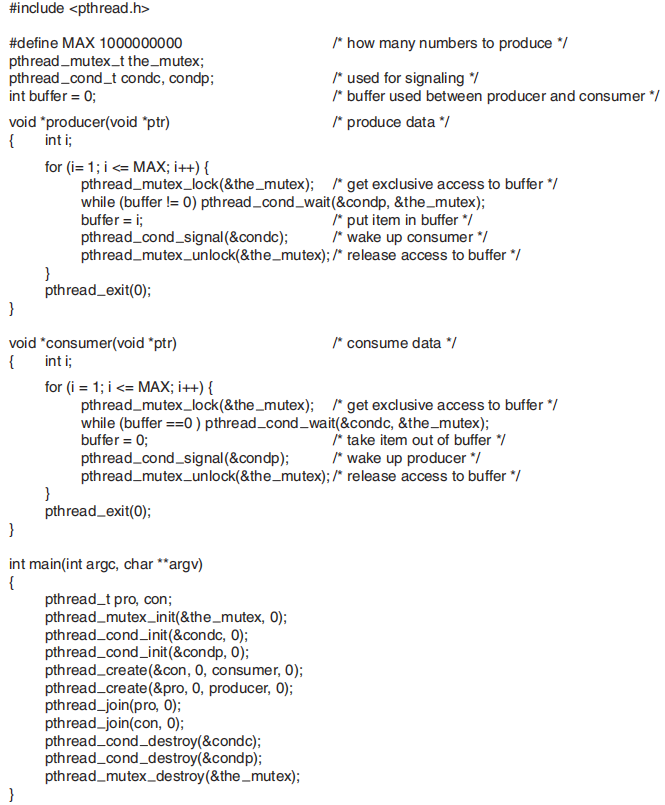
\includegraphics[width=0.90\textwidth]{FIG/2-32.png}
		\caption{一个使用线程来解决生产者和消费者问题的例子} \label{fig:thread-producer-consumer}
	\end{figure}
	
	\subsection{管程}
	
	有了信号量和互斥量之后,进程间的通信好像很简单了,事实上是这样的吗?你想多了。请仔细地考察向缓冲区放入数据项以及从缓冲区中删除数据项之前的down操作。假设在生产者的代码中两个\texttt{down}操作的顺序反了,所以\texttt{mutex}在变\texttt{empty}之前减少了而不是在它之后减少的。如果缓冲区是完全满的,生产者将会阻塞,\texttt{mutex}被设置为0。结果,当下次消费者想要访问缓冲区,它将对\texttt{mutex}执行减操作,现在已经是0了,因此也被阻塞。两个进程将会拥有地阻塞,并且不能再做其他任何的工作了,这种不幸的情形称为死锁,我们将在第6章中详细介绍死锁。
	
	指出这个问题是因为在使用信号量的时候必须多加小心,稍有不慎,一切都会戛然而止。这就像使用汇编语言编程,甚至更糟,因为这里出现的情况都是条件竞争,死锁等不可预见和不可重现的错误。
	
	为了使得编写正确的程序容易一些,Brinch Hansen(1973)和Hoare(1974)提出了一个称为管程(monitor)的高级同步原语。在下面的介绍中,他们两人提出的方案略有不同。一个管程是在一类特殊的模块或包中组合在一起的一个过程,变量和数据结构的集合。进程可以在它们想要的任何时候调用管程中的过程,但是它们不能通过声明在管程之外的过程来访问管程内部的数据结构。图 \ref{fig:monitor} 展示了一种抽象的,类Pascal语言编写的管程。C语言不能在这里使用,因为管程是一个语言概念,而C语言并不支持它。
	 
	\begin{figure}[ht]\small
		\centering
		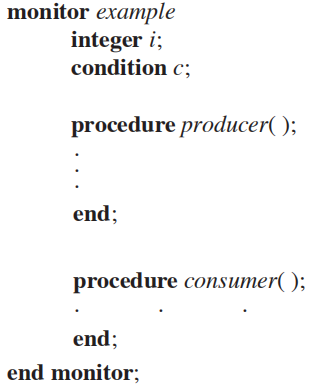
\includegraphics[width=0.90\textwidth]{FIG/2-33.png}
		\caption{一个管程}\label{fig:monitor}
	\end{figure}

	管程有一个重要的特征,这使得它们有利于实现互斥:在任意时刻,管程中只有一个进程是活跃的。管程是一种编程语言结构,因为编译器知道它是特殊的,可以处理不同于其他过程调用的管程过程的调用。典型地,当一个进程调用了管程过程,该过程的前几条指令将检查监视器中当前是否有其他进程处于活动状态。如果是,调用线程将挂起直到其他的线程离开管程为止。如果没有其他的进程使用管程,调用进程将可以进入。
	由编译器在管程条目上实现互斥,但一种常见的方法是使用互斥或二进制信号量。因为是编译器,而不是编程语言,在处理互斥,因此出错误的概率要小得多。在任何时刻,编写管程的人都不需要知道编译器是如何安排互斥量的。只要知道将所有关键区域转换为管程,就不会有两个过程同时执行它们的临界区。
	尽管管程提供了一个实现互斥的简单方式,就像我们看到的那样,这还是不够的。我们还需要一个当进程不能继续的时候可以阻塞的方法。在生产者和消费者问题中,很容易将针对缓冲区满和缓冲区空的测试放置到管程中,但是在生产者发现缓冲区满的时候该如何阻塞呢?
	
	解决方案在于引入条件变量,以及对它们的两个操作wait和signal。当一个管程发现它不能继续的时候(生产者发现缓冲区满了),它对一些条件变量(如full)执行一个\texttt{wait}操作。这个动作导致调用进程阻塞。它还允许以前禁止进入监视器的进程现在进入。在前面介绍Pthread时候我们已经看到条件变量及其操作了。
	
	另一个进程(例如,消费者)可以通过对其伙伴正在等待的条件变量执行一个信号来唤醒其睡眠伙伴。为了避免管程中同时活动的两个进程,我们需要一个规则来告诉在一个信号后将会发生什么。Hoare提出的方法是让新唤醒的进程运行,挂起另外一个进程。Brinch-Hansen提出了如果一个进程发送了一个发送信号的请求,则它必须立即退出管程的方法来解决这个问题。
	
	换句话说,一个\texttt{signal}语句可能是在管程中的最后一个语句。这里将采纳Brinch-Hansen的方案,因为它在概念上更加地简单,并且更容易实现。如果一个信号是在一个条件变量上完成的,其中有几个进程正在等待,则只有其中一个进程由系统调度器确定。
	
	顺便提一下,还有一个不是由Hoare或者Brinch Hansen提出的第三种方案。这是为了让signaler继续运行,并允许等待进程仅在信号器退出管程后才开始运行。
	
	条件变量不是计数器,它们不会像信号量那样为以后的使用积累信号。所以,如果像一个条件变量发送信号,但是该条件变量上并没有等待线程,则该信号就会永远地丢失。换句话说,\texttt{wait}操作必须在\texttt{signal}之前,这条规则使得实现简单了很多。
	实际上,这不是一个问题,因为在需要的时候,很容易使用变量来跟踪每一个进程的状态。一个可能会发出一个信号的进程可以通过查看变量来发现这个操作是不必要的。
	
	一个使用类Pascal语言编写的带有管程的生产者消费者问题的框架在图 \ref{fig:monitor-producer-consumer} 中给出。
	
	\begin{figure}[ht]\small
		\centering
		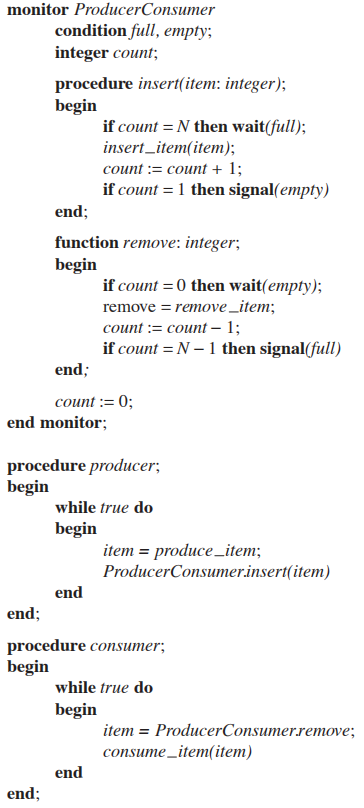
\includegraphics[width=0.90\textwidth]{FIG/2-34.png}
		\caption{一个使用管程的生产者和消费者问题。在一个时刻只有一个管程过程是活动的。缓冲区有N个槽位。}\label{fig:monitor-producer-consumer}
	\end{figure}

	生产者和消费者线程的功能和之前所有例子中的部分都是类似的。生产者有一个无限循环生成数据并把它放置到公共缓冲区,消费者同样有一个无限循环将数据取出缓冲区并做一些有趣的事情。
	
	
	
	
	
	
	
	
	
	
	
	
		
	
	
	
	
	
	
	
		
	
	
	
	
	
	
	
	
	
	
	
	
	
	
	
	
	
	
	
	
	
	
	
	
	
	
	
	
	
	
	
	
	
	
	
	
	
	
	
	
	

	
	
	
	
	
	
	
	
	
	
	
	
	
	
	
	
	
	
	
	
	

%\setlength{\fboxrule}{0pt}\setlength{\fboxsep}{0cm}
%\noindent\shadowbox{
%\begin{tcolorbox}[arc=0mm,colback=lightblue,colframe=darkblue,title=学习目标与要求]
%\kai\textcolor{darkblue}{1.~~了解科学计算的一般过程.}\\
%\kai\textcolor{darkblue}{2.~~了解数值计算方法的研究内容和特点.}\\
%\kai\textcolor{darkblue}{3.~~理解数值计算误差的有关概念.}\\
%\kai\textcolor{darkblue}{4.~~掌握数值计算误差的控制方法.}
%\end{tcolorbox}}
%\setlength{\fboxrule}{1pt}\setlength{\fboxsep}{4pt}
%
%
%\section{Colored boxes}
%
%\begin{tcolorbox}[colback=red!5,colframe=red!75!black]
%  My box.
%\end{tcolorbox}
%
%\begin{tcolorbox}[colback=blue!5,colframe=blue!75!black,title=My title]
%  My box with my title.
%\end{tcolorbox}
%
%\begin{tcolorbox}[colback=green!5,colframe=green!75!black]
%  Upper part of my box.
%  \tcblower
%  Lower part of my box.
%\end{tcolorbox}
%
%\begin{tcolorbox}[colback=yellow!5,colframe=yellow!75!black,title=My title]
%  I can do this also with a title.
%  \tcblower
%  Lower part of my box.
%\end{tcolorbox}
%
%\begin{tcolorbox}[colback=yellow!10,colframe=red!75!black,lowerbox=invisible,
%  savelowerto=\jobname_ex.tex]
%  Now, we play hide and seek. Where is the lower part?
%  \tcblower
%  I'm invisible until you find me.
%\end{tcolorbox}
%
%\begin{tcolorbox}[colback=yellow!10,colframe=red!75!black,title=Here I am]
%  \input{\jobname_ex.tex}
%\end{tcolorbox}
%
%
%\begin{tcolorbox}[colback=blue!50,colframe=blue!25!black,coltext=yellow,
%    fontupper=\Large\bfseries,arc=6mm,boxrule=2mm,boxsep=5mm]
%  ofFunny settings.
%\end{tcolorbox}
%
%\subsection{\LaTeX-Table}
%
%\begin{table}[h]\begin{center}\color{darkblue}\caption{计算结果}\color{black}\label{tab1-2}
%{\footnotesize
%\begin{tabular}{r|r||r|r||r|r||r|r}\arrayrulecolor{darkblue}\hline\rowcolor{lightblue}
%  $n$&$I_n$&$n$&$I_n$&$n$&$I_n$&$n$&$I_n$\\\hline
%  19&0.008\ 3&14&0.011\ 2&9&0.016\ 9&4&0.034\ 3\\
%  18&0.008\ 9&13&0.012\ 0&8&0.018\ 8&3&0.043\ 1\\
%  17&0.009\ 3&12&0.013\ 0&7&0.021\ 2&2&0.058\ 0\\
%  16&0.009\ 9&11&0.014\ 1&6&0.024\ 3&1&0.088\ 4\\
%  15&0.010\ 5&10&0.015\ 4&5&0.028\ 5&0&0.182\ 3\\\hline
% \end{tabular}}\end{center}\end{table}
%
%
%\section{\LaTeX-Examples}
%
%\begin{tcblisting}{colback=red!5,colframe=red!75!black}
%This is a \LaTeX\ example:
%$\displaystyle\sum\limits_{i=1}^n i = \frac{n(n+1)}{2}$.
%\end{tcblisting}
%
%
%\section{Theorems}
%
%\begin{defi}{Summation of Numbers}{defi1.1}
%  For all natural number $n$ it holds:\\[2mm]
%  $\displaystyle\sum\limits_{i=1}^n i = \frac{n(n+1)}{2}$.
%\end{defi}
%
%\begin{theo}{Summation of Numbers}{theo1.1}
%  For all natural number $n$ it holds:\\[2mm]
%  $\displaystyle\sum\limits_{i=1}^n i = \frac{n(n+1)}{2}$.
%\end{theo}
%
%\begin{coro}{Summation of Numbers}{coro1.1}
%  For all natural number $n$ it holds:\\[2mm]
%  $\displaystyle\sum\limits_{i=1}^n i = \frac{n(n+1)}{2}$.
%\end{coro}
%We have given Theorem \ref{Theorem:theo1.1} on page \pageref{Theorem:theo1.1}.
%
%
%
%\begin{table}[h]\begin{center}\color{darkblue}\caption{计算结果}\color{black}\label{tab1-1}
%{\footnotesize
%\begin{tabular}{r|r||r|r||r|r||r|r}\arrayrulecolor{darkblue}\hline\rowcolor{lightblue}
%  $n$&$I_n$&$n$&$I_n$&$n$&$I_n$&$n$&$I_n$\\\hline
%  1&0.088\ 4&6&0.034\ 4&11&-31.392\ 5&16&9.814\ 5e+4\\
%  2&0.581\ 0&7&-0.029\ 0&12&157.045\ 7&17&-4.907\ 3e+5\\
%  3&0.043\ 1&8&0.270\ 1&13&-785.151\ 6&18&2.453\ 6e+6\\
%  4&0.347\ 0&9&-1.239\ 3&14&3.925\ 8e+3&19&-1.226\ 8e+7\\
%  5&0.026\ 5&10&0.296\ 7&15&-1.962\ 9e+4&20&6.134\ 1e+7\\\hline
%\end{tabular}}\end{center}\end{table}
%
%\section{graphicx}
%
%\begin{figure}[h]
%\begin{minipage}[t]{0.5\linewidth}
%\centering
%%\includegraphics[totalheight=1.2in]{fig/tu2-2}
%\caption{不动点迭代法收敛} \label{fig:tu2-2}
%\end{minipage}
%\begin{minipage}[t]{0.5\linewidth}
%\centering
%%\includegraphics[totalheight=1.3in]{fig/tu2-3}
%\caption{不动点迭代法发散} \label{fig:tu2-3}
%\end{minipage}
%\end{figure}
%
%
%
%\vspace{0.5cm}
%\addcontentsline{toc}{section}{\protect\numberline{}{习题一}}
%\markboth{习题一}{习题一} \centerline{\textcolor{darkblue}{\hei\zihao{4}
% 习题一}}\vspace{0.5cm}
%
%
